\chapter{Groups and Group Functions}
\label{chap:group_function}
\markboth{Groups and Group Functions}{Groups and Group Functions}

\begin{remark}[Positioning of this chapter]\label{rem:group_function_chapter_positioning}
Starting from the axioms of group representation theory, this chapter builds up the theoretical system of group actions, the three standard constructions on a group (translation, inner automorphism, outer automorphism), group symmetry, group direction, group periods and the space of group functions.

The chapter has three core tasks:
\begin{enumerate}[label=(\arabic*)]
    \item \textbf{Defining the eight pairs of concepts}: translation function/translation group, scaling function/scaling group, rotation function/rotation group, conservation function/conservation group, symmetry function/symmetry group, closure function/closure group, periodic function/group with periodic orbits, higher-order function/higher-order group.
    \item \textbf{Establishing the joint phase-space criterion framework}: unifying the closure criterion for phase-space trajectories with the criterion for groups with periodic orbits from group representation theory, and giving a complete criterion for the periodicity of a function.
    \item \textbf{Proving the transitivity matrix}: for the transitivity of the eight properties under the twelve operations (addition, subtraction, multiplication, division, exponentiation, root extraction, logarithm, series, limits, differentiation, integration, convolution), giving a proof or a counterexample cell by cell.
\end{enumerate}

\textbf{Note}: the three standard constructions on a group---left translation $L_g$, right translation $R_g$, inner automorphism $\iota_g$ and the outer automorphism group $\operatorname{Out}(G)$---are respectively classical objects in group representation theory. This chapter treats them as independent objects of group representation theory.

Seven-theme guide for this chapter: Translation---left/right translation on a group (the centre of symmetry being the identity element $e$); Scaling---the outer automorphism $\operatorname{Out}(G)$; Rotation---the inner automorphism $\iota_g$ (the centre of symmetry being the centre $Z(G)$); Conservation---the conservation laws of group functions (translation invariance$\to$momentum/energy, scaling invariance$\to$scale charge, rotation invariance$\to$angular momentum); Symmetry---the automorphism tower and the groupification of relations; Closure---the closure of group orbits and the criteria for the eight pairs of concepts; Period---group periods and groups with periodic orbits.
\end{remark}

\begin{figure}[htbp]
\centering
\begin{tikzpicture}[
  node distance=7mm and 10mm,
  box/.style={draw, rounded corners, align=center, minimum width=2.6cm, minimum height=0.75cm, fill=blue!5, font=\small},
  core/.style={draw, very thick, rounded corners, align=center, minimum width=3.4cm, minimum height=0.95cm, fill=orange!15},
  arrow/.style={-{Stealth[length=2mm]}, thick}
]
\node[core] (core) {Groups and group functions\\unified algebraic framework};
\node[box, above left=of core] (trans) {Translation\\left/right regular action};
\node[box, above right=of core] (rot) {Rotation\\inner automorphism $\iota_g$};
\node[box, right=of core] (scal) {Scaling\\outer automorphism $\operatorname{Out}(G)$};
\node[box, below left=of core] (tower) {Automorphism tower\\$\operatorname{Aut}^k(G)$};
\node[box, below=of core] (concept) {Eight pairs of concepts\\translation/scaling/rotation/$\cdots$};
\node[box, below right=of core] (matrix) {Transitivity matrix\\8 properties $\times$ 12 operations};
\foreach \x in {trans,rot,scal,tower,concept,matrix}
  \draw[arrow] (core) -- (\x);
\end{tikzpicture}
\caption{Overall roadmap of the `Groups and Group Functions' chapter: the three standard constructions, the automorphism tower, the eight pairs of concepts and the transitivity matrix together constitute a unified algebraic framework.}
\label{fig:group_function_overview}
\end{figure}

\section{\texorpdfstring{The Three Standard Constructions on a Group}{The Three Standard Constructions on a Group}}

On a vector space, vector addition (translation), the outer product/complex multiplication (rotation) and scalar multiplication (scaling) are three basic operations, and they stand in a formal correspondence with the gradient, the curl and the divergence (centre of symmetry $1$) respectively. This section generalises this viewpoint to an arbitrary group: on any group there likewise exist three standard constructions---left/right translation, inner automorphism and outer automorphism---which are the counterparts of the above three operations at the level of group representation theory. In the discussion that follows, the `three constructions' are classical objects of group representation theory; the `correspondence with the three operators' is an organising viewpoint whose rigour depends on the particular context.

\subsection{\texorpdfstring{Translation Construction}{Translation Construction}}

\begin{definition}[Translation Construction on a Group]\label{def:group_translation_operation}
Let $(G,\cdot)$ be a group. For each fixed $g \in G$, define two mappings:
\begin{itemize}
    \item \textbf{Left translation} $L_g: G \to G$: $L_g(x) = g \cdot x$, $\forall x \in G$.
    \item \textbf{Right translation} $R_g: G \to G$: $R_g(x) = x \cdot g$, $\forall x \in G$.
\end{itemize}
Left and right translation have the following properties:
\begin{enumerate}[label=(\roman*)]
    \item The set of left translations $\{L_g : g \in G\}$ forms a group under composition of mappings, with $L_g \circ L_h = L_{gh}$ and $L_{g^{-1}} = (L_g)^{-1}$. This group is isomorphic to $G$ itself and is called the \textbf{left regular action} of $G$.
    \item The set of right translations forms a group, with $R_g \circ R_h = R_{hg}$, isomorphic to $G^{\text{op}}$ (the opposite group of $G$).
    \item Left and right translations commute with each other: $L_g \circ R_h = R_h \circ L_g$ (because $(gx)h = g(xh)$).
\end{enumerate}
\end{definition}

\begin{figure}[htbp]
\centering
\begin{tikzpicture}[>=Stealth, thick, scale=1.0]
\draw[->] (-0.3,0) -- (7.5,0) node[right] {$G$};
\foreach \x/\l in {0.5/e, 2.0/x, 4.5/gx, 6.5/g} {
  \fill (\x,0) circle (1.5pt);
}
\node[below] at (0.5,-0.1) {$e$};
\node[below] at (2.0,-0.1) {$x$};
\node[below] at (4.5,-0.1) {$gx$};
\node[below] at (6.5,-0.1) {$g$};
\draw[->, blue, very thick] (2.0,0.25) -- (4.5,0.25);
\node[blue, above] at (3.25,0.35) {$L_g$};
\draw[->, red, very thick] (4.5,-0.25) -- (6.5,-0.25);
\node[red, below] at (5.5,-0.35) {$L_g$};
\draw[->, green!60!black, very thick] (6.5,0.6) -- (2.0,0.6);
\node[green!60!black, above] at (4.2,0.7) {$L_{g^{-1}}$};
\node at (3.5,-1.5) {Left translation $L_g(x)=gx$ is an isometric translation acting from the identity element side};
\end{tikzpicture}
\qquad
\begin{tikzpicture}[>=Stealth, thick, scale=1.0]
\draw[->] (-0.3,0) -- (7.5,0) node[right] {$G$};
\foreach \x/\l in {0.5/e, 2.0/x, 4.0/xg, 6.0/g} {
  \fill (\x,0) circle (1.5pt);
}
\node[below] at (0.5,-0.1) {$e$};
\node[below] at (2.0,-0.1) {$x$};
\node[below] at (4.0,-0.1) {$xg$};
\node[below] at (6.0,-0.1) {$g$};
\draw[->, red, very thick] (2.0,0.25) -- (4.0,0.25);
\node[red, above] at (3.0,0.35) {$R_g$};
\draw[->, blue, very thick] (6.0,-0.25) -- (2.0,-0.25);
\node[blue, below] at (4.0,-0.35) {$R_{g^{-1}}$};
\node at (3.5,-1.5) {Right translation $R_g(x)=xg$ is an isometric translation acting from the side opposite to the identity};
\end{tikzpicture}
\caption{Comparison of left translation $L_g$ with right translation $R_g$. When $G$ is non-commutative the two are in general unequal, but $L_g\circ R_h=R_h\circ L_g$ always holds.}
\label{fig:left_right_translation}
\end{figure}

\begin{proposition}[Basic Properties of the Translation Construction]\label{prop:translation_operator}
The translation construction on a group (left translation and right translation) has the following properties:
\begin{enumerate}[label=(\roman*)]
    \item \textbf{Fixed elements}: the identity element $e$ of the group satisfies $L_g(e) = g$ and $R_g(e) = g$. The inversion mapping $\sigma_e(x) = x^{-1}$ is an involution ($\sigma_e \circ \sigma_e = \operatorname{id}_G$).
    \item \textbf{Infinitesimal generators}: when $G$ is a Lie group, the infinitesimal generator of left translation is a \textbf{left-invariant vector field}, whose differential operator corresponds to an element of the Lie algebra $\mathfrak{g}$. For $G = \mathbb{R}$ (the additive group), the infinitesimal generator is $\frac{d}{dx}$. For $G = \mathbb{R}^n$ (the additive group), the infinitesimal generators are $(\partial_1, \dots, \partial_n)$.
    \item \textbf{Invariance of the Haar measure}: translation invariance is expressed as the left invariance of the Haar measure: $\int_G f(gx) dg = \int_G f(x) dg$. By Noether's theorem, translation invariance implies the conservation of momentum or energy.
    \item \textbf{Directional structure}: each generator $g \in G$ defines a `translation direction'---moving group elements along that direction. For a discrete group this is manifested as directed edges of the Cayley graph.
\end{enumerate}
\end{proposition}

\begin{proof}
(i) For any $x \in G$, $\sigma_e(\sigma_e(x)) = (x^{-1})^{-1} = x$, so $\sigma_e$ is an involution. $L_g(e) = g \cdot e = g$ and $R_g(e) = e \cdot g = g$.

(ii) For a Lie group $G$, the left-invariant vector field $\tilde{X}(g) = dL_g|_e(X)$ ($X \in \mathfrak{g}$) generates the one-parameter subgroup of left translations: $\exp(tX) \cdot g = L_{\exp(tX)}(g)$. For $G = \mathbb{R}$ the Lie algebra $\mathfrak{g} \cong \mathbb{R}$ is one-dimensional, and the left-invariant vector field corresponding to the basis vector $X = 1$ is $\tilde{X}(x) = \frac{d}{dx}$, which generates the translation $x \mapsto x + t$.

(iii) The left invariance of the Haar measure is the integral expression of translation invariance. By Noether's theorem, translation invariance implies the conservation of momentum/energy.

(iv) For a discrete group, the generating set $S$ defines the basic translation directions. For a Lie group, the basis $\{X_1, \dots, X_n\}$ of the Lie algebra defines $n$ independent translation directions.
\end{proof}

\begin{example}[Examples of the Translation Construction]\label{ex:translation_operation_examples}
\begin{itemize}
    \item \textbf{The additive group of integers $\mathbb{Z}$}: left translation $L_n(m) = n+m$. The generator $1$ defines the positive direction ($+1$), and the generator $-1$ defines the negative direction. For example $L_3(5)=3+5=8$ and $L_{-2}(1)=-1$. The conserved quantity is the discrete momentum.
    \item \textbf{The additive group of real numbers $\mathbb{R}$}: left translation $L_a(x) = a+x$. The infinitesimal generator is $\frac{d}{dx}$, and its exponential mapping $\exp\big(t\frac{d}{dx}\big)$ acting on $x$ gives $x+t$ (taking $t=\frac12$: $L_{1/2}(0)=\frac12$). The conserved quantity is the continuous momentum (or energy, when $x$ is a time parameter).
    \item \textbf{The general linear group $GL(n,\mathbb{R})$}: left translation $L_A(X) = AX$ (matrix multiplication). This is the realisation of the translation construction on a non-commutative group.
\end{itemize}
\end{example}

\subsection{\texorpdfstring{Inner Automorphism}{Inner Automorphism}}
\label{subsec:inner_automorphism}

\begin{definition}[Inner Automorphism]\label{def:group_rotation_operation}
For each fixed $g \in G$, define the mapping $\iota_g: G \to G$ by
\[
\iota_g(x) = g x g^{-1}, \quad \forall x \in G.
\]
$\iota_g$ is called the \textbf{inner automorphism} determined by $g$ (or the conjugation mapping). Inner automorphisms have the following properties:
\begin{enumerate}[label=(\roman*)]
    \item $\iota_g$ is an automorphism of $G$: it is a bijection (with inverse mapping $\iota_{g^{-1}}$) and preserves the group operation: $\iota_g(xy) = g(xy)g^{-1} = (gxg^{-1})(gyg^{-1}) = \iota_g(x)\iota_g(y)$.
    \item The mapping $G \to \operatorname{Aut}(G)$, $g \mapsto \iota_g$ is a group homomorphism whose kernel is the \textbf{centre} $Z(G) = \{z \in G : gz = zg,\ \forall g \in G\}$ of $G$.
    \item The inner automorphisms as a whole form a normal subgroup of $\operatorname{Aut}(G)$, written $\operatorname{Inn}(G) \cong G/Z(G)$.
\end{enumerate}
\end{definition}

\begin{proposition}[Basic Properties of the Inner Automorphism]\label{prop:rotation_operator}
Inner automorphisms on a group have the following properties:
\begin{enumerate}[label=(\roman*)]
    \item \textbf{Fixed elements}: the elements of the centre $Z(G)$. For any $z \in Z(G)$, $\iota_z(x) = zxz^{-1} = x$ (because $zx = xz$), that is, the elements of $Z(G)$ are fixed under conjugation. For $G = U(1)$ (an Abelian group), $Z(U(1)) = U(1)$, and all elements are fixed elements.
    \item \textbf{Infinitesimal generators}: when $G$ is a Lie group, the infinitesimal generator of an inner automorphism is the \textbf{adjoint representation} $\operatorname{ad}_X(Y) = [X,Y]$ (the Lie bracket of the Lie algebra). For $G = U(1)$ the Lie algebra $\mathfrak{u}(1) \cong i\mathbb{R}$ is a one-dimensional commutative Lie algebra and the adjoint representation is zero ($[X,Y]=0$). For $G = SO(3)$ the adjoint representation gives the Lie-algebra version of the angular momentum operator.
    \item \textbf{Conserved quantities}: conjugation invariance implies the \textbf{conservation of angular momentum}. At the level of group representation theory this is manifested as the invariance of class functions under conjugation: $f(gxg^{-1}) = f(x)$. The character $\chi_\rho$ is a typical example of a class function.
    \item \textbf{Adjoint orbits}: each non-central element $g \in G \setminus Z(G)$ defines a `rotation direction'---conjugating group elements along that direction. For $G = U(1)$ (an Abelian group) all inner automorphisms are the identity mapping. For a non-commutative group the rotation directions are given by the adjoint orbits.
\end{enumerate}
\end{proposition}

\begin{proof}
(i) If $z \in Z(G)$, then for any $x \in G$, $\iota_z(x) = zxz^{-1} = xzz^{-1} = x$. For $G = U(1)$ the multiplication is commutative, so $Z(U(1)) = U(1)$.

(ii) For a Lie group $G$, the infinitesimal generator of the inner automorphism $\iota_{\exp(tX)}$ as $t \to 0$ is $\operatorname{ad}_X(Y) = \frac{d}{dt}\big|_{t=0} \iota_{\exp(tX)}(\exp(Y)) = [X,Y]$. For $G = U(1)$ the Lie algebra is one-dimensional and commutative, $[X,Y]=0$, and the adjoint representation is trivial. For $G = SO(3)$ the Lie algebra $\mathfrak{so}(3) \cong \mathbb{R}^3$ is equipped with the cross product as Lie bracket, and $\operatorname{ad}_X(Y) = X \times Y$.

(iii) A class function $f(gxg^{-1}) = f(x)$ is invariant under conjugation. The character $\chi_\rho(g) = \operatorname{Tr}(\rho(g))$ satisfies $\chi_\rho(gxg^{-1}) = \operatorname{Tr}(\rho(g)\rho(x)\rho(g)^{-1}) = \operatorname{Tr}(\rho(x)) = \chi_\rho(x)$, and is therefore a class function.

(iv) For a non-commutative group, the adjoint orbit $\mathcal{O}_x = \{gxg^{-1} : g \in G\}$ gives the orbit structure of $x$ under inner automorphisms. The size of the orbit is given by the orbit-stabiliser theorem: $|\mathcal{O}_x| = |G|/|C_G(x)|$, where $C_G(x) = \{g \in G : gx = xg\}$ is the centraliser of $x$.
\end{proof}

\begin{figure}[htbp]
\centering
\begin{tikzpicture}[>=Stealth, thick, scale=1.0]
\draw[thick, dashed] (0,0) circle (1.8);
\draw[thick, dashed] (0,0) circle (0.9);
\fill (0,0) circle (2pt) node[below right] {$Z(G)$};
\foreach \a in {20, 80, 140, 200, 260, 320} {
  \fill (\a:1.8) circle (1.8pt);
  \fill (\a:0.9) circle (1.8pt);
}
\draw[->, red, very thick] (20:1.8) to[bend left=20] (80:1.8);
\draw[->, red, very thick] (80:1.8) to[bend left=20] (200:1.8);
\node[red] at (1.0,2.3) {Conjugacy orbit $\mathcal{O}_x$};
\node[blue] at (-4.5,0) {each element of $Z(G)$ forms an orbit by itself};
\end{tikzpicture}
\caption{Orbit structure of an inner automorphism: the conjugation action partitions $G$ into conjugacy classes (orbits), each element of the centre $Z(G)$ forms an orbit by itself, and a class function takes a constant value on each orbit.}
\label{fig:inner_automorphism_orbits}
\end{figure}

\begin{example}[Examples of the Inner Automorphism]\label{ex:rotation_operation_examples}
\begin{itemize}
    \item \textbf{The general linear group $GL(n,\mathbb{R})$}: the inner automorphism $\iota_A(X) = AXA^{-1}$ is the similarity transformation of matrices. Two matrices are similar if and only if they lie in the same adjoint orbit. For example, conjugating $A=\begin{pmatrix}2&0\\0&1\end{pmatrix}$ by the permutation matrix $P=\begin{pmatrix}0&1\\1&0\end{pmatrix}$ gives $\iota_P(A)=PAP^{-1}=\begin{pmatrix}1&0\\0&2\end{pmatrix}$, whose eigenvalues $\{1,2\}$ are invariant under conjugation.
    \item \textbf{The three-dimensional rotation group $SO(3)$}: the inner automorphism $\iota_R(S) = RSR^{-1}$ conjugates the rotation $S$ into a rotation about a new axis. Two rotations are conjugate if and only if they have the same rotation angle (the same eigenvalues).
    \item \textbf{The circle group $U(1)$} (an Abelian group): all inner automorphisms are the identity mapping, and inner automorphisms degenerate to the trivial one.
\end{itemize}
\end{example}

\subsection{\texorpdfstring{Outer Automorphism}{Outer Automorphism}}
\label{subsec:outer_automorphism}

\begin{definition}[Outer Automorphism Group]\label{def:group_scaling_operation}
The quotient group $\operatorname{Out}(G) = \operatorname{Aut}(G) / \operatorname{Inn}(G)$ is called the \textbf{outer automorphism group} of $G$. The elements of $\operatorname{Out}(G)$ represent those automorphisms that cannot be realised by conjugation by elements of the group.

Typical examples of outer automorphisms include:
\begin{enumerate}[label=(\roman*)]
    \item \textbf{Automorphisms of a cyclic group}: $\operatorname{Aut}(C_n) \cong (\mathbb{Z}/n\mathbb{Z})^\times$, the automorphisms being $x \mapsto x^k$ ($\gcd(k,n)=1$). When $k \neq \pm 1$ this is not an inner automorphism (because $C_n$ is an Abelian group, all of whose inner automorphisms are the identity mapping), and hence belongs to the outer automorphism group.
    \item \textbf{Automorphisms of the additive group of integers}: $\operatorname{Aut}(\mathbb{Z}) \cong C_2 = \{\operatorname{id}, -\operatorname{id}\}$, and the negation mapping $x \mapsto -x$ is the only non-trivial automorphism.
    \item \textbf{Outer automorphisms of the general linear group}: $\operatorname{Aut}(GL(n,\mathbb{R}))$ contains the inverse-transpose mapping $X \mapsto (X^{\mathsf T})^{-1}$ (a non-trivial outer automorphism when $n \ge 3$), together with diagonal automorphisms and so on.
\end{enumerate}
\end{definition}

\begin{proposition}[Basic Properties of the Outer Automorphism]\label{prop:scaling_operator}
Outer automorphisms on a group have the following properties:
\begin{enumerate}[label=(\roman*)]
    \item \textbf{Fixed elements}: the set of fixed elements of an automorphism $\varphi \in \operatorname{Aut}(G)$ of the group is $\{x \in G : \varphi(x) = x\}$, which is a subgroup. For the automorphism $x \mapsto x^k$ of a cyclic group, the set of fixed points is $\{x \in C_n : x^{k-1} = e\}$, that is, the subgroup consisting of the elements whose order divides $k-1$. For the negation mapping in $\operatorname{Aut}(\mathbb{Z})$, the only fixed point is $0$.
    \item \textbf{Infinitesimal generators}: outer automorphisms are not generated by conjugation by elements of the group, and therefore have no `infinitesimal generator' at the level of group representation theory (they do not arise from the adjoint action of the Lie algebra). For $G = \mathbb{R}$ (the additive group), the infinitesimal generator of the automorphism $x \mapsto \lambda x$ ($\lambda \neq 0$) is $x \frac{d}{dx}$.
    \item \textbf{Invariants}: automorphisms keep the structure constants of the group unchanged. For the automorphism $x \mapsto x^k$ of a cyclic group, it keeps the order of the group unchanged ($|G|$ is conserved).
    \item \textbf{Directional structure}: outer automorphisms do not change the conjugacy-class structure among group elements, but they change the overall scale of the group.
\end{enumerate}
\end{proposition}

\begin{proof}
(i) For the cyclic group $C_n = \langle g \rangle$, the automorphism is $\varphi_k(g^m) = g^{km}$ ($\gcd(k,n)=1$). Fixed points satisfy $g^{km} = g^m \iff g^{m(k-1)} = e \iff n \mid m(k-1)$. When $\gcd(k-1,n) = d$, the fixed points form the subgroup of order $d$ generated by $g^{n/d}$.

(ii) For $G = \mathbb{R}$ (the additive group), the automorphisms are $\varphi_\lambda(x) = \lambda x$ ($\lambda \in \mathbb{R}^\times$). The tangent vector at $\lambda = 1$ is $\frac{d}{d\lambda}\big|_{\lambda=1} \varphi_\lambda(x) = x$, to which the differential operator $x \frac{d}{dx}$ corresponds.

(iii) Automorphisms preserve the order of the group: $|\varphi(G)| = |G|$ (because $\varphi$ is a bijection). For a cyclic group this means that $|C_n| = n$ is invariant under automorphisms.

(iv) What outer automorphisms change is the `external structure' of the group---they cannot be realised by conjugation by elements of the group, yet they preserve the conjugacy-class structure (the conjugacy classes are intrinsic invariants of the group).
\end{proof}

\begin{figure}[htbp]
\centering
\begin{tikzpicture}[>=Stealth, thick, scale=1.0]
\draw[->] (-0.3,0) -- (7,0) node[right] {$\mathbb{R}$};
\foreach \x in {0.5, 2.0, 3.5, 5.0, 6.5} \fill (\x,0) circle (1.5pt);
\draw[<->, blue, very thick] (2.0,0.4) -- (5.0,0.4);
\node[blue, above] at (3.5,0.5) {$\varphi_\lambda: x\mapsto \lambda x$};
\draw[<->, red, very thick] (2.0,-0.4) -- (5.0,-0.4);
\node[red, below] at (3.5,-0.5) {scale invariance: $|C_n|$ unchanged};
\node at (3.5,-1.4) {outer automorphisms change the scale but not the conjugacy-class structure};
\end{tikzpicture}
\caption{Geometric intuition for outer automorphisms: the ring-like arrows represent the scaling transformation $x \mapsto \lambda x$, and the two ends of the arrow correspond to the property that the group order is unchanged.}
\label{fig:outer_automorphism_scaling}
\end{figure}

\begin{example}[Examples of the Outer Automorphism]\label{ex:scaling_operation_examples}
\begin{itemize}
    \item \textbf{The additive group of integers $\mathbb{Z}$}: $\operatorname{Aut}(\mathbb{Z}) \cong C_2 = \{\operatorname{id}, -\operatorname{id}\}$. The negation mapping is $x \mapsto -x$, for example $-3 \mapsto 3$. The only fixed point is $0$.
    \item \textbf{The cyclic group $C_n$}: $\operatorname{Aut}(C_n) \cong (\mathbb{Z}/n\mathbb{Z})^\times$, of order $\varphi(n)$ (the Euler function). The automorphism $x \mapsto x^k$ ($\gcd(k,n)=1$) rescales the generator. For example, when $n=5$, $\operatorname{Aut}(C_5)\cong(\mathbb{Z}/5\mathbb{Z})^\times\cong C_4$, and the generator $g$ is mapped in turn to $g^1,g^2,g^3,g^4$ under $\varphi_k(g)=g^k$ ($k=1,2,3,4$).
    \item \textbf{The multiplicative group of positive real numbers $\mathbb{R}^+$}: $\operatorname{Aut}(\mathbb{R}^+) \cong \mathbb{R}^\times$. The automorphism $x \mapsto x^\lambda$ is a power scaling.
\end{itemize}
\end{example}

\subsection{The Unified Structure of the Three Constructions}

\begin{theorem}[The Unification Theorem for the Three Constructions on a Group]\label{thm:three_operations_unity}
Let $G$ be a group. The three standard constructions on a group have the following structure in the automorphism group $\operatorname{Aut}(G)$:
\begin{enumerate}[label=(\roman*)]
    \item \textbf{Translation construction}: realised by $G$ itself through the left regular action, with the operating group isomorphic to $G$. The set of translation operations $\{L_g : g \in G\}$ is a faithful action of $G$ on itself.
    \item \textbf{Inner automorphisms}: realised by the inner automorphism group $\operatorname{Inn}(G) \cong G/Z(G)$. $\operatorname{Inn}(G)$ is a normal subgroup of $\operatorname{Aut}(G)$.
    \item \textbf{Outer automorphisms}: realised by the outer automorphism group $\operatorname{Out}(G) = \operatorname{Aut}(G)/\operatorname{Inn}(G)$.
\end{enumerate}
In the automorphism tower $G_{(0)} = G, G_{(1)} = \operatorname{Aut}(G), G_{(2)} = \operatorname{Aut}(\operatorname{Aut}(G)), \dots$, every level contains that level's translation, inner automorphism and outer automorphism constructions.
\end{theorem}

\begin{proof}
(i) The left regular action $\lambda: G \to \operatorname{Sym}(G)$, $\lambda(g) = L_g$, is a group homomorphism. Its kernel is $\{e\}$, hence it is faithful.

(ii) The inner automorphism $\iota_g(x) = gxg^{-1}$ is an automorphism and preserves the group operation. The kernel of the mapping $G \to \operatorname{Aut}(G)$, $g \mapsto \iota_g$ is $Z(G)$, hence $\operatorname{Inn}(G) \cong G/Z(G)$. $\operatorname{Inn}(G)$ is a normal subgroup of $\operatorname{Aut}(G)$.

(iii) $\operatorname{Out}(G) = \operatorname{Aut}(G)/\operatorname{Inn}(G)$ is a quotient group.
\end{proof}

\begin{figure}[htbp]
\centering
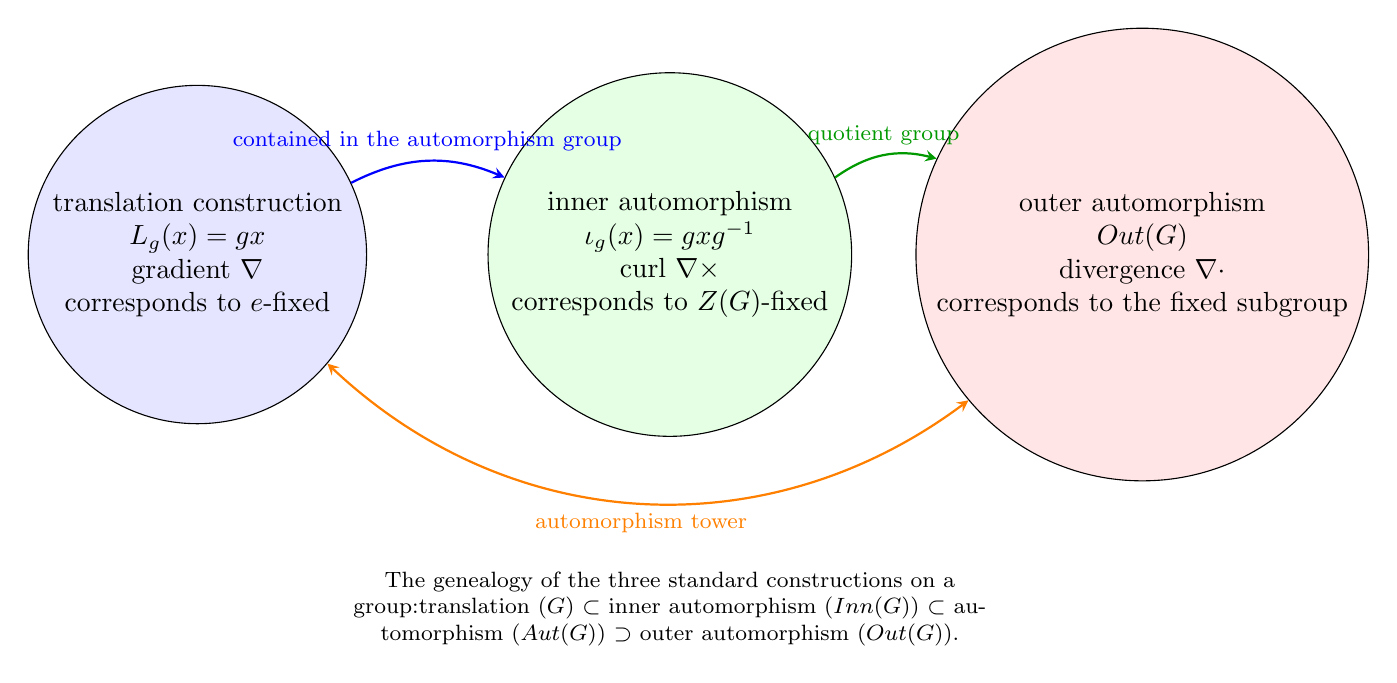
\begin{tikzpicture}[scale=1.0, >=stealth]

\node[draw, circle, fill=blue!10, minimum size=2.5cm, align=center]
  (trans) at (0,0)
  {translation construction\\$L_g(x)=gx$\\gradient $\nabla$\\corresponds to $e$-fixed};

\node[draw, circle, fill=green!10, minimum size=2.5cm, align=center]
  (rot) at (6,0)
  {inner automorphism\\$\iota_g(x)=gxg^{-1}$\\curl $\nabla\times$\\corresponds to $Z(G)$-fixed};

\node[draw, circle, fill=red!10, minimum size=2.5cm, align=center]
  (scal) at (12,0)
  {outer automorphism\\$\operatorname{Out}(G)$\\divergence $\nabla\cdot$\\corresponds to the fixed subgroup};

\draw[->, thick, blue]
  (trans) to[bend left=25]
  node[above, font=\footnotesize] {contained in the automorphism group}
  (rot);

\draw[->, thick, green!60!black]
  (rot) to[bend left=25]
  node[above, font=\footnotesize] {quotient group}
  (scal);

\draw[<->, thick, orange]
  (scal) to[bend left=40]
  node[below, font=\footnotesize] {automorphism tower}
  (trans);

\node[font=\footnotesize, text width=0.9\textwidth, align=center]
  at (6, -4.5)
  {The genealogy of the three standard constructions on a group:%
   translation ($G$) $\subset$ inner automorphism ($\operatorname{Inn}(G)$)
   $\subset$ automorphism ($\operatorname{Aut}(G)$)
   $\supset$ outer automorphism ($\operatorname{Out}(G)$).};

\end{tikzpicture}
\vspace{1cm}
\caption{A unified perspective on the three standard constructions on a group.}
\label{fig:three_operations_unity}
\end{figure}

\section{\texorpdfstring{The Automorphism Tower}{The Automorphism Tower}}
\label{sec:automorphism_tower}

\begin{definition}[Automorphism of a Group]\label{def:automorphism}
Let $(G,\cdot)$ be a group. A mapping $\varphi: G \to G$ is called an \textbf{automorphism} of $G$ if it is a bijection and preserves the group operation: $\varphi(xy) = \varphi(x)\varphi(y)$.
\end{definition}

\begin{definition}[The Automorphism Group]\label{def:automorphism_group}
The automorphisms of $G$ as a whole form a group under composition of mappings, written $\operatorname{Aut}(G)$. The identity element is the identity mapping and the inverse element is the inverse mapping.
\end{definition}

\begin{proposition}[The Inverse of an Automorphism Preserves the Group Operation]\label{prop:automorphism_inverse}
Let $\varphi \in \operatorname{Aut}(G)$. Then its inverse mapping $\varphi^{-1}$ also preserves the group operation.
\end{proposition}

\begin{proof}
Since $\varphi$ is surjective, there exist unique $x, y \in G$ such that $\varphi(x) = u$ and $\varphi(y) = v$. By the homomorphism property of $\varphi$, $\varphi(xy) = uv$. Applying $\varphi^{-1}$ to both sides gives $xy = \varphi^{-1}(uv)$. But $xy = \varphi^{-1}(u)\varphi^{-1}(v)$, hence $\varphi^{-1}(uv) = \varphi^{-1}(u)\varphi^{-1}(v)$.
\end{proof}

\begin{definition}[Inner Automorphism]\label{def:inner_automorphism}
This definition is the same content as that given in Chapter~\ref{chap:group_function} (the `Inner Automorphism' section, \cref{subsec:inner_automorphism}), namely \cref{def:group_rotation_operation}; to avoid repeated exposition, only the reference anchor is retained here, and the complete statement is to be found there.
\end{definition}

\begin{definition}[The Outer Automorphism Group]\label{def:outer_automorphism}
This definition is the same content as that given in Chapter~\ref{chap:group_function} (the `Outer Automorphism' section, \cref{subsec:outer_automorphism}), namely \cref{def:group_scaling_operation}; to avoid repeated exposition, only the reference anchor is retained here, and the complete statement is to be found there.
\end{definition}

\begin{definition}[The Automorphism Tower]\label{def:automorphism_tower}
Define recursively $G_{(0)} = G$ and $G_{(k+1)} = \operatorname{Aut}(G_{(k)})$. Level $0$ is the group itself, level $1$ is the automorphism group, level $2$ is the automorphism group of the automorphism group, and so on. On every level $G_{(k)}$ there exist three standard constructions: translation (the left regular action), inner automorphisms ($\operatorname{Inn}(G_{(k)})$) and outer automorphisms ($\operatorname{Out}(G_{(k)})$).
\end{definition}

\begin{figure}[htbp]
\centering
\begin{tikzpicture}[>=Stealth, thick, node distance=1.6cm, scale=0.95]
\node[draw, rounded corners, fill=blue!8, align=center] (g0) at (0,0) {$G_{(0)}=G$};
\node[draw, rounded corners, fill=green!8, align=center] (g1) at (4,0) {$G_{(1)}=\operatorname{Aut}(G)$};
\node[draw, rounded corners, fill=orange!8, align=center, text width=0.8\textwidth] (g2) at (8,0) {$G_{(2)}=\operatorname{Aut}^2(G)$};
\node[align=center] (gdots) at (11.5,0) {$\cdots$};
\draw[->] (g0) -- (g1);
\draw[->] (g1) -- (g2);
\draw[->, dashed] (g2) -- (gdots);
\foreach \x/\y/\name in {0/-1.6/translation, 4/-1.6/translation, 8/-1.6/translation} {
  \node[font=\footnotesize] at (\x,\y) {\name};
}
\foreach \x/\y/\name in {0/-2.2/inner automorphism, 4/-2.2/inner automorphism, 8/-2.2/inner automorphism} {
  \node[font=\footnotesize] at (\x,\y) {\name};
}
\foreach \x/\y/\name in {0/-2.8/outer automorphism, 4/-2.8/outer automorphism, 8/-2.8/outer automorphism} {
  \node[font=\footnotesize] at (\x,\y) {\name};
}
\node at (5.5,-3.8) {every level $G_{(k)}$ again possesses the three constructions: translation / inner automorphism / outer automorphism};
\end{tikzpicture}
\caption{Level-by-level structure of the automorphism tower: each level is the automorphism group of the level below, and the three standard constructions reappear on every level.}
\label{fig:automorphism_tower}
\end{figure}

\begin{lemma}[Embedding and Equal-Order Stability for Centreless Groups]\label{ch8_centreless_embedding}
Let $G$ be a finite group with $Z(G)=\{e\}$. Then
\begin{enumerate}[label=(\roman*)]
    \item the inner automorphism mapping $G\to\operatorname{Aut}(G)$, $g\mapsto\iota_g$, is a monomorphism, hence $G\cong\operatorname{Inn}(G)\subseteq\operatorname{Aut}(G)$, and therefore $|G|\le|\operatorname{Aut}(G)|$;
    \item if $|\operatorname{Aut}(G)|=|G|$, then $\operatorname{Aut}(G)=\operatorname{Inn}(G)\cong G$;
    \item $Z(\operatorname{Aut}(G))=\{e\}$, that is, triviality of the centre is preserved level by level in the automorphism tower.
\end{enumerate}
\end{lemma}

\begin{proof}
(i) The kernel of the mapping $g\mapsto\iota_g$ is $Z(G)=\{e\}$ (Definition \ref{def:inner_automorphism}), so it is a monomorphism with image $\operatorname{Inn}(G)$, whence $G\cong\operatorname{Inn}(G)\subseteq\operatorname{Aut}(G)$.

(ii) By (i), $\operatorname{Inn}(G)\subseteq\operatorname{Aut}(G)$ and $|\operatorname{Inn}(G)|=|G|=|\operatorname{Aut}(G)|$, hence $\operatorname{Inn}(G)=\operatorname{Aut}(G)$; moreover $\operatorname{Inn}(G)\cong G/Z(G)=G$, so $\operatorname{Aut}(G)\cong G$.

(iii) Let $\psi\in Z(\operatorname{Aut}(G))$. Then $\psi\iota_g=\iota_g\psi$ for all $g$, that is, $\psi(gxg^{-1})=g\psi(x)g^{-1}$. Since $\psi$ is a homomorphism, $\psi(g)\psi(x)\psi(g)^{-1}=g\psi(x)g^{-1}$, so $\psi(g)^{-1}g$ commutes with $\psi(x)$. Since $\psi$ is surjective, $\psi(x)$ runs through all of $G$, hence $\psi(g)^{-1}g\in Z(G)=\{e\}$, that is, $\psi(g)=g$ for all $g$, and therefore $\psi=\operatorname{id}$. Hence $Z(\operatorname{Aut}(G))=\{e\}$.
\end{proof}

\begin{theorem}[Stability of the Automorphism Tower of a Finite Group---Wielandt's Theorem]\label{thm:finite_automorphism_tower}
Let $G$ be a finite group with trivial centre $Z(G)$. Then the automorphism tower stabilises in finitely many steps: there exists $N \in \mathbb{N}$ such that $G_{(k+1)} \cong G_{(k)}$ for every $k \ge N$.
\end{theorem}

\begin{proof}
By (i) and (iii) of Lemma \ref{ch8_centreless_embedding}, by induction every level $G_{(k)}$ is centreless, and $G_{(k)}\cong\operatorname{Inn}(G_{(k)})\subseteq G_{(k+1)}$, so $|G_{(k+1)}|\ge|G_{(k)}|$; by (ii) again, equality holds if and only if $G_{(k+1)}\cong G_{(k)}$, that is, the tower stabilises at $k$. If the tower never terminates, the sequence $|G_{(k)}|$ is strictly increasing. The core assertion of Wielandt (1939) is that the orders in the automorphism tower of a centreless finite group are bounded above (the bound depending only on $G$), so a strictly increasing process cannot continue indefinitely and must stop after finitely many steps; combined with the fact that equal orders imply stability, the tower stabilises identically after finitely many steps.
\end{proof}

\begin{remark}[The Boundary of Wielandt's Theorem]\label{rem:wielandt_boundary}
The three steps given by Lemma \ref{ch8_centreless_embedding}---`the order is monotonically non-decreasing + equal orders imply stability + triviality of the centre is preserved level by level'---can be proved entirely self-containedly; the boundedness of the order (a strict increase must terminate), however, is a classical result of Wielandt (1939) whose complete proof is rather long, and it is cited here as a known theorem. When the centre is non-trivial the automorphism tower need not stabilise in finitely many steps (counterexamples can be constructed), so the `trivial centre' hypothesis in the theorem cannot be omitted.
\end{remark}

\section{\texorpdfstring{Group Actions and Symmetry}{Group Actions and Symmetry}}

\begin{definition}[Group Action]\label{def:group_action_gf}
Let $G$ be a group and $X$ a non-empty set. A \textbf{left action} of $G$ on $X$ is a mapping $\Phi: G \times X \to X$ satisfying:
\begin{enumerate}[label=(\roman*)]
    \item \textbf{Identity action}: $\Phi(e, x) = x$ for all $x \in X$;
    \item \textbf{Associativity}: $\Phi(g, \Phi(h, x)) = \Phi(gh, x)$ for all $g,h \in G$ and $x \in X$.
\end{enumerate}
One usually writes $\Phi(g, x)$ as $g \cdot x$.
\end{definition}

\begin{definition}[Orbit and Stabiliser Subgroup]\label{def:orbit_stabilizer}
Let the group $G$ act on the set $X$. For any $x \in X$:
\begin{itemize}
    \item $G \cdot x := \{g \cdot x : g \in G\}$ is called the \textbf{orbit} of $x$.
    \item $G_x := \{g \in G : g \cdot x = x\}$ is called the \textbf{stabiliser subgroup} of $x$.
\end{itemize}
\end{definition}

\begin{theorem}[The Orbit-Stabiliser Theorem]\label{thm:orbit_stabilizer}
Let a finite group $G$ act on a finite set $X$. For any $x \in X$,
\[
|G \cdot x| = \frac{|G|}{|G_x|}.
\]
\end{theorem}

\begin{proof}
Consider the mapping $\varphi: G \to G \cdot x$, $\varphi(g) = g \cdot x$. This mapping is surjective. $\varphi(g_1) = \varphi(g_2)$ if and only if $g_2^{-1}g_1 \in G_x$, equivalently $g_1 G_x = g_2 G_x$. Hence $\varphi$ induces a one-to-one correspondence from $G/G_x$ onto $G \cdot x$.
\end{proof}

\begin{figure}[htbp]
\centering
\begin{tikzpicture}[>=Stealth, thick, scale=1.0]
\draw[fill=blue!5] (-3,-2.0) rectangle (7,3.0);
\node[blue] at (5.6,2.1) {$X$};
\draw[fill=green!8] (0,0.5) ellipse (1.3 and 0.85);
\node at (0,0.5) {$G\cdot x$};
\fill (0,0.5) circle (2pt) node[below right, font=\footnotesize] {$x$};
\draw[fill=red!8] (4.5,0.5) ellipse (1.1 and 0.75);
\node at (4.5,0.5) {$G\cdot y$};
\fill (4.5,0.5) circle (2pt) node[below right, font=\footnotesize] {$y$};
\node at (-2.0,0.5) {$G_x$};
\draw[->, red, very thick] (0,-0.5) -- (0,-1.2);
\node at (0,-1.6) {$|G\cdot x|=|G|/|G_x|$};
\node at (4.5,-1.6) {$|G\cdot y|=|G|/|G_y|$};
\end{tikzpicture}
\caption{The orbit-stabiliser theorem: the group $G$ acts on the set $X$, and the size of each orbit equals the order of the group divided by the order of the stabiliser subgroup of the point.}
\label{fig:orbit_stabilizer}
\end{figure}

\section{\texorpdfstring{Group Symmetry and Group Direction}{Group Symmetry and Group Direction}}

\begin{definition}[Translational Symmetry on a Group]\label{def:group_translation_symmetry}
Translational symmetry on a group $G$ is the group action formed by left and right translations.
\end{definition}

\begin{definition}[Automorphism Symmetry on a Group]\label{def:group_automorphism_symmetry}
Automorphism symmetry on a group $G$ is the natural action of $\operatorname{Aut}(G)$ on $G$: $\varphi \cdot x = \varphi(x)$. It includes inner automorphisms ($\operatorname{Inn}(G)$) and outer automorphisms ($\operatorname{Out}(G)$).
\end{definition}

\begin{proposition}[Compatibility of Translation and Automorphism]\label{prop:translation_automorphism_compatibility}
Let $\varphi \in \operatorname{Aut}(G)$ and $g \in G$. Then
\[
\varphi \circ L_g \circ \varphi^{-1} = L_{\varphi(g)}.
\]
\end{proposition}

\begin{proof}
For any $x \in G$: $(\varphi \circ L_g \circ \varphi^{-1})(x) = \varphi(g \cdot \varphi^{-1}(x)) = \varphi(g) \cdot x = L_{\varphi(g)}(x)$.
\end{proof}

\begin{definition}[Directional Structure of a Discrete Group]\label{def:discrete_group_direction}
Let $G$ be a finitely generated group and $S \subseteq G$ a symmetric generating set ($S = S^{-1}$, $\langle S \rangle = G$). The \textbf{directional structure} on $G$ is given by the Cayley graph $\Gamma(G,S)$: the vertex set is $G$, and for each $g \in G$ and $s \in S$ there is a directed edge from $g$ to $gs$.
\end{definition}

\begin{definition}[Directional Structure of a Lie Group]\label{def:lie_group_direction}
Let $G$ be a Lie group and $\mathfrak{g} = T_e G$ its Lie algebra. Each non-zero element $X$ of $\mathfrak{g}$ determines a \textbf{left-invariant vector field} $\tilde{X}(g) = dL_g|_e(X)$. A basis $\{X_1, \dots, X_n\}$ of the Lie algebra gives a set of \textbf{basic directions} on the group.
\end{definition}

\begin{proposition}[Algebraic Structure of Left-Invariant Vector Fields]\label{prop:left_invariant_fields}
Let $\tilde{X}, \tilde{Y}$ be left-invariant vector fields. Then $[\tilde{X}, \tilde{Y}]$ is also a left-invariant vector field, and $[\tilde{X}, \tilde{Y}] = \widetilde{[X,Y]}$.
\end{proposition}

\begin{proof}
$[\tilde{X}, \tilde{Y}](g) = dL_g|_e([X,Y]) = \widetilde{[X,Y]}(g)$.
\end{proof}

\begin{figure}[htbp]
\centering
\begin{tikzpicture}[>=Stealth, thick, scale=0.95]
\node[draw, circle, fill=blue!8, minimum size=1.4cm] (g) at (0,0) {$g$};
\foreach \a/\n in {60/gs_1, 120/gs_2, 180/gs_3, 240/gs_4, 300/gs_5, 0/gs_6} {
  \node[draw, circle, fill=blue!4, minimum size=1.0cm] (\n) at (\a:2.4) {};
}
\draw[->] (g) -- (gs_1);
\draw[->] (g) -- (gs_2);
\draw[->] (g) -- (gs_3);
\draw[->] (g) -- (gs_4);
\draw[->] (g) -- (gs_5);
\draw[->] (g) -- (gs_6);
\node at (0,-3.5) {Cayley graph $\Gamma(G,S)$: each generator $s\in S$ corresponds to a directed edge};
\end{tikzpicture}
\qquad
\begin{tikzpicture}[>=Stealth, thick, scale=0.95]
\draw[thick] (0,0) .. controls (1,0.8) and (2,-0.8) .. (3,0);
\draw[->, red, very thick] (0.1,0.1) -- (0.5,0.4);
\draw[->, red, very thick] (1.4,0.4) -- (1.8,0.1);
\draw[->, red, very thick] (2.6,-0.3) -- (2.9,0.0);
\node[red] at (1.5,1.1) {left-invariant vector field $\tilde X(g)=dL_g|_e(X)$};
\node at (1.5,-1.1) {the Lie algebra basis $\{X_i\}$ gives the basic directions};
\end{tikzpicture}
\caption{Comparison of the directional structure of a discrete group (left) with that of a Lie group (right): the directed edges of the Cayley graph correspond to left-invariant vector fields.}
\label{fig:group_directions}
\end{figure}

\section{\texorpdfstring{Definitions of the Eight Pairs of Concepts}{Definitions of the Eight Pairs of Concepts}}
\label{sec:group_function_basic}

\subsection{\texorpdfstring{Translation Functions and the Translation Group}{Translation Functions and the Translation Group}}

\begin{definition}[Translation Function]\label{def:translation_function_gf}
Let $\mathcal{D} = \mathbb{R}$, $f: \mathcal{D} \to V$, $G = (\mathbb{R}, +)$, with group action $\phi_a(x) = x + a$. If there exists $a_0 \neq 0$ such that $f(x + a_0) = f(x)$ for all $x \in \mathcal{D}$, then $f$ is called a \textbf{translation function} with respect to the translation $a_0$.
\end{definition}

\begin{definition}[Translation Group]\label{def:translation_group_gf}
The \textbf{translation group} of a translation function $f$ is defined as
\[
\operatorname{Translation}(f) = \{a \in \mathbb{R} : f(x + a) = f(x),\; \forall x \in \mathcal{D}\}.
\]
$\operatorname{Translation}(f)$ is necessarily either $\{0\}$ or some $T\mathbb{Z}$ ($T>0$); for its structure and that of the quotient space $\mathbb{R}/\operatorname{Translation}(f)\cong S^1$, see Proposition \ref{prop:invariance_subgroup_structure}.
\end{definition}

\subsection{\texorpdfstring{Scaling Functions and the Scaling Group}{Scaling Functions and the Scaling Group}}

\begin{definition}[Scaling Function]\label{def:scaling_function_gf}
Let $\mathcal{D} = \mathbb{R}^+$, $f: \mathcal{D} \to V$, $G = (\mathbb{R}^+, \times)$, with group action $\phi_q(x) = qx$. If there exists $q_0 > 0, q_0 \neq 1$ such that $f(q_0 x) = f(x)$ for all $x \in \mathcal{D}$, then $f$ is called a \textbf{scaling function} with respect to the scaling $q_0$.
\end{definition}

\begin{definition}[Scaling Group]\label{def:scaling_group_gf}
The \textbf{scaling group} of a scaling function $f$ is defined as
\[
\operatorname{Scaling}(f) = \{q \in \mathbb{R}^+ : f(qx) = f(x),\; \forall x \in \mathcal{D}\}.
\]
$\operatorname{Scaling}(f)$ is necessarily either $\{1\}$ or some $\langle q_0\rangle$ ($q_0>1$); under the logarithm mapping $\ln$ it is isomorphic to an additive subgroup of $(\mathbb{R},+)$. For its structure see Proposition \ref{prop:invariance_subgroup_structure}.
\end{definition}

\subsection{\texorpdfstring{Rotation Functions and the Rotation Group}{Rotation Functions and the Rotation Group}}

\begin{definition}[Rotation Function]\label{def:rotation_function_gf}
Let $\mathcal{D} = \mathbb{C}$, $f: \mathcal{D} \to V$, $G = U(1)$, with group action $\phi_\theta(z) = e^{i\theta}z$. If there exists $\theta_0 \neq 0$ such that $f(e^{i\theta_0} z) = f(z)$ for all $z \in \mathcal{D}$, then $f$ is called a \textbf{rotation function} with respect to the rotation $e^{i\theta_0}$.
\end{definition}

\begin{definition}[Rotation Group]\label{def:rotation_group_gf}
The \textbf{rotation group} of a rotation function $f$ is defined as
\[
\operatorname{Rotation}(f) = \{e^{i\theta} \in U(1) : f(e^{i\theta}z) = f(z),\; \forall z \in \mathcal{D}\}.
\]
$\operatorname{Rotation}(f)$ is necessarily either a finite cyclic group $C_q$ or the whole of $U(1)$; note that `the cyclic subgroup generated by a single rotation' and `the group formed by all rotational symmetries' are two different things, see Proposition \ref{prop:invariance_subgroup_structure} and Remark \ref{rem:rotation_dense_corrected}.
\end{definition}

\subsection{\texorpdfstring{Conservation Functions and the Conservation Group}{Conservation Functions and the Conservation Group}}

\begin{definition}[Conservation Function]\label{def:conservation_function_gf}
Let $f: \mathcal{D} \to V$ and let $G$ be a group acting on $\mathcal{D}$. $f$ is called a \textbf{conservation function} with respect to $G$ if there exists a scalar functional $Q: V \to \mathbb{R}$ (a \textbf{conserved quantity}) such that
\[
Q(f(\phi_g(x))) = Q(f(x)), \quad \forall g \in G,\; \forall x \in \mathcal{D}.
\]
Conservation and symmetry always appear together: symmetry is invariance under a transformation, and conservation is the quantitative expression of that invariance.
\end{definition}

\begin{definition}[Conservation Group]\label{def:conservation_group_gf}
The conservation group (equivariance group) was first defined in Chapter~\ref{chap:period_foundation} \cref{sec:invariants_conservation}, \cref{def:conservation_group}; the present form is its expression in the notation of the group function $f$ and the quantity $Q$.
The \textbf{conservation group} of a conservation function $f$ is defined as
\[
\operatorname{Group}_{\mathrm{conservation}}(f, Q) = \{g \in G : Q(f(\phi_g(x))) = Q(f(x)),\; \forall x \in \mathcal{D}\}.
\]
The symmetry group is contained in the conservation group: $\operatorname{Symmetry}(f) \subseteq \operatorname{Group}_{\mathrm{conservation}}(f, Q)$.
\end{definition}

\subsection{\texorpdfstring{Symmetry Functions and the Symmetry Group}{Symmetry Functions and the Symmetry Group}}

\begin{definition}[Symmetry Function]\label{def:symmetry_function_gf}
$f$ is called a \textbf{symmetry function} with respect to $g \in G$ if $f(\phi_g(x)) = f(x)$ for all $x \in \mathcal{D}$. A symmetry function is a special case of a conservation function (the conserved quantity $Q$ being taken to be the identity functional).
\end{definition}

\begin{definition}[Symmetry Group]\label{def:symmetry_group_gf}
The \textbf{symmetry group} of a symmetry function $f$ is defined as
\[
\operatorname{Symmetry}(f) = \{g \in G : f(\phi_g(x)) = f(x),\; \forall x \in \mathcal{D}\}.
\]
The group with periodic orbits $\operatorname{Group}_{\mathrm{period}}(f) = \operatorname{Symmetry}(f)$.
\end{definition}

\subsection{\texorpdfstring{Closure Functions and the Closure Group}{Closure Functions and the Closure Group}}

\begin{definition}[Closure Function]\label{def:closure_function_gf}
Let $f: \mathcal{D} \to V$ be a smooth function. $f$ is called a \textbf{closure function} with respect to $g \in G$ if, in the \textbf{phase space} $T^*\mathcal{D}$, the phase-space trajectory $\Gamma_f(x) = (f(x), \dot{f}(x))$ of $f$ is closed under the action of $\phi_g$: $\Gamma_f(\phi_g(x)) = \Gamma_f(x)$.
\end{definition}

\begin{definition}[Closure Group]\label{def:closure_group_gf}
The \textbf{closure group} of a closure function $f$ is defined as
\[
\operatorname{Clos}(f) = \{g \in G : \Gamma_f(\phi_g(x)) = \Gamma_f(x),\; \forall x \in \mathcal{D}\}.
\]
$\operatorname{Group}_{\mathrm{period}}(f) \subseteq \operatorname{Clos}(f)$---a periodic function is necessarily a closure function.
\end{definition}

\subsection{\texorpdfstring{Periodic Functions and the Group with Periodic Orbits}{Periodic Functions and the Group with Periodic Orbits}}

\begin{definition}[Periodic Function]\label{def:periodic_function_gf}
$f$ is called a \textbf{periodic function} with respect to $g \in G$ if $f(\phi_g(x)) = f(x)$ for all $x \in \mathcal{D}$. A periodic function is equivalent to a function on the quotient space $\mathcal{D}/\operatorname{Group}_{\mathrm{period}}(f)$.
\end{definition}

\begin{definition}[Group with Periodic Orbits]\label{def:group_with_periodic_orbits_gf}
The \textbf{group with periodic orbits} of a periodic function $f$ is defined as
\[
\operatorname{Group}_{\mathrm{period}}(f) = \{g \in G : f(\phi_g(x)) = f(x),\; \forall x \in \mathcal{D}\}.
\]
\end{definition}

\subsection{\texorpdfstring{Higher-Order Functions and the Higher-Order Group}{Higher-Order Functions and the Higher-Order Group}}

\begin{definition}[Higher-Order Function]\label{def:higher_function_gf}
Let $f: G \to V$ be a group function. The \textbf{higher-order functions} of $f$ are the sequence of functions on the levels of the automorphism tower: $f_{(0)} = f$, $f_{(k)}: G_{(k)} \to V$, $k \ge 1$.
\end{definition}

\begin{definition}[Higher-Order Group]
\label{def:higher_group_gf}
The \textbf{higher-order group} of $G$ refers to its automorphism tower
\[
G_{(0)} = G,\quad
G_{(1)} = \operatorname{Aut}(G),\quad
G_{(2)} = \operatorname{Aut}(\operatorname{Aut}(G)),\;\dots
\]
\end{definition}

\begin{table}[htbp]
    \centering
    \caption{Comparison table of the eight pairs of concepts and the formally corresponding operators}
    \label{tab:eight_concept_pairs}
    \begin{tabular}{>{\centering\arraybackslash}p{2.2cm}>{\centering\arraybackslash}p{2.2cm}>{\centering\arraybackslash}p{2cm}>{\centering\arraybackslash}p{2cm}>{\centering\arraybackslash}p{2.5cm}>{\centering\arraybackslash}p{2.5cm}}
        \toprule
        Function concept & Group concept & Formally corresponding operator & Fixed element & Formally corresponding conserved quantity & Phase-space criterion \\
        \midrule
        Translation function & Translation group & Gradient $\nabla$ & $0$ & Momentum/energy & The phase trajectory closes along the translation axis \\
        Scaling function & Scaling group & Divergence $\nabla\cdot$ & $1$ & Scale charge & The phase trajectory closes in the logarithmic domain \\
        Rotation function & Rotation group & Curl $\nabla\times$ & $i$ & Angular momentum & The phase trajectory closes about the rotation axis \\
        Conservation function & Conservation group & The three operators & $0,1,i$ & The corresponding conserved quantity & The conserved quantity is invariant in phase space \\
        Symmetry function & Symmetry group & The three operators & $0,1,i$ & The corresponding conserved quantity & The symmetry transformation preserves the phase trajectory \\
        Closure function & Closure group & The three operators & $0,1,i$ & The corresponding conserved quantity & The phase-space trajectory is closed \\
        Periodic function & Group with periodic orbits & The three operators & $0,1,i$ & The corresponding conserved quantity & Configuration + phase space close simultaneously \\
        Higher-order function & Higher-order group & Automorphism tower & Level by level & Level-by-level conservation & Phase space on the automorphism tower \\
        \bottomrule
    \end{tabular}
\end{table}

\begin{figure}[htbp]
\centering
\begin{tikzpicture}[>=Stealth, thick, node distance=8mm, scale=0.95]
\node[draw, rounded corners, fill=blue!8, align=center] (period) {Periodic function\\$\operatorname{Group}_{\mathrm{period}}(f)$};
\node[draw, rounded corners, fill=green!8, align=center, below=of period] (sym) {Symmetry function\\$\operatorname{Symmetry}(f)$};
\node[draw, rounded corners, fill=orange!8, align=center, below=of sym] (cons) {Conservation function\\$\operatorname{Group}_{\mathrm{conservation}}(f,Q)$};
\node[draw, rounded corners, fill=red!8, align=center, below=of cons] (clos) {Closure function\\$\operatorname{Clos}(f)$};
\node[draw, rounded corners, fill=purple!8, align=center, left=2.2cm of sym] (trans) {Translation function};
\node[draw, rounded corners, fill=purple!8, align=center, right=2.2cm of sym] (rot) {Rotation function};
\node[draw, rounded corners, fill=purple!8, align=center, right=2.2cm of cons] (scal) {Scaling function};
\node[draw, rounded corners, fill=yellow!12, align=center, below=1.0cm of clos] (high) {Higher-order function\\$f_{(k)}:G_{(k)}\to V$};
\draw[->] (period) -- (sym);
\draw[->] (sym) -- (cons);
\draw[->] (clos) -- (cons);
\draw[->] (trans) -- (sym);
\draw[->] (rot) -- (sym);
\draw[->] (scal) -- (cons);
\draw[->] (clos) -- (high);
\end{tikzpicture}
\caption{Hierarchical structure of the eight pairs of concepts: translation / scaling / rotation are concrete invariance subgroups, period, symmetry, conservation and closure form a unified chain of inclusions, and higher-order functions are further sublimated through the automorphism tower.}
\label{fig:eight_concept_pairs_hierarchy}
\end{figure}

\begin{proposition}[Structure of the three invariance subgroups]\label{prop:invariance_subgroup_structure}
Let $f:\mathcal{D}\to V$ be \textbf{continuous and non-constant}, and let the three actions be $\phi_a(x)=x+a$ ($\mathcal{D}=\mathbb{R}$), $\phi_q(x)=qx$ ($\mathcal{D}=\mathbb{R}^+$) and $\phi_\theta(z)=e^{i\theta}z$ ($\mathcal{D}=\mathbb{C}^\times$) respectively. Then
\begin{enumerate}[label=(\roman*)]
    \item \textbf{Translation}: $\operatorname{Translation}(f)$ is a closed subgroup of $(\mathbb{R},+)$, hence is either $\{0\}$ or $T\mathbb{Z}$ for some $T>0$; in the latter case $\mathcal{D}/\operatorname{Translation}(f)\cong\mathbb{R}/T\mathbb{Z}\cong S^1$.
    \item \textbf{Scaling}: $\operatorname{Scaling}(f)$ is a closed subgroup of $(\mathbb{R}^+,\times)$, hence is either $\{1\}$ or $\langle q_0\rangle$ for some $q_0>1$.
    \item \textbf{Rotation}: $\operatorname{Rotation}(f)$ is a closed subgroup of $U(1)$, hence is either a finite cyclic group $C_q$ for some $q\ge1$, or the whole of $U(1)$; when $\operatorname{Rotation}(f)=U(1)$, $f$ depends only on $|z|$, that is, $f$ is a \textbf{radial function}.
\end{enumerate}
\end{proposition}

\begin{proof}
\textbf{Subgroup property}: the three sets are closed under their respective group operations, contain the identity element and contain inverses (the latter following from the invariance of $f$ under the identity transformation), hence all three are subgroups.

\textbf{Closedness}: taking translation as an example, let $a_n\in\operatorname{Translation}(f)$ with $a_n\to a$. For any $x$, by the continuity of $f$,
\[
f(x+a)=\lim_{n\to\infty}f(x+a_n)=\lim_{n\to\infty}f(x)=f(x),
\]
hence $a\in\operatorname{Translation}(f)$. The scaling and rotation cases are analogous (using the continuity of multiplication and the topology of $U(1)$ respectively).

(i) The closed subgroups of $(\mathbb{R},+)$ are only $\{0\}$ and $\alpha\mathbb{Z}$ ($\alpha>0$): this is the classical classification of the one-dimensional subgroups of $(\mathbb{R},+)$---if a closed subgroup $H\neq\{0\}$, take $T:=\inf\{h\in H:h>0\}$; by closedness $T\in H$; if $H\neq T\mathbb{Z}$, then there exists $h\in H$ whose ratio to $T$ is irrational, in which case $H$ is dense in $\mathbb{R}$, and by closedness $H=\mathbb{R}$. Taking $T$ then gives the least positive element. The isomorphism of quotient spaces is given by $x+T\mathbb{Z}\mapsto e^{2\pi ix/T}$.

(ii) $\ln:(\mathbb{R}^+,\times)\to(\mathbb{R},+)$ is a homeomorphism and a group isomorphism; it maps $\operatorname{Scaling}(f)$ onto a closed subgroup of $(\mathbb{R},+)$ and maps $q_0>1$ to $\ln q_0>0$. The result follows from (i).

(iii) A closed subgroup of $U(1)$ is either discrete or $U(1)$ itself; a discrete closed subgroup consists of roots of unity, that is, it is some $C_q$. If $\operatorname{Rotation}(f)=U(1)$, then $f$ is invariant under all rotations; writing $z\neq0$ in polar form $z=|z|e^{i\arg z}$, rotational invariance allows us to take $\arg z=0$, hence $f(z)=f(|z|)$.
\end{proof}

\begin{remark}[The correct statement concerning `denseness']\label{rem:rotation_dense_corrected}
Proposition \ref{prop:invariance_subgroup_structure}(iii) contains a point that is very easily confused and requires separate explanation:
\begin{enumerate}[label=(\roman*)]
    \item if $\theta_0/(2\pi)=p/q$ (in lowest terms), then the cyclic subgroup generated by the single rotation $e^{i\theta_0}$ is $C_q$ (finite and closed), and $\operatorname{Rotation}(f)\supseteq C_q$;
    \item if $\theta_0/(2\pi)\notin\mathbb{Q}$, then the cyclic subgroup generated by $e^{i\theta_0}$ is infinite and \textbf{dense in $U(1)$}; but it is \textbf{not closed}, and therefore is \textbf{not equal to} $\operatorname{Rotation}(f)$.
\end{enumerate}
In other words: \textbf{`denseness' is a property of the generated subgroup, not a property of the invariance subgroup}. As a closed subgroup, $\operatorname{Rotation}(f)$ has only two possibilities: some finite cyclic group $C_q$, or the whole of $U(1)$. Calling the rotation symmetry group of $f$ `dense' is inaccurate.
\end{remark}

\begin{remark}[On the group relations of the eight pairs of concepts]\label{rem:concept_pair_relations}
The following four items are consequences of notational conventions and of a single substitution, and are relations at the level of definitions; they are therefore given in the form of a remark rather than as a proposition:
\begin{enumerate}[label=(\roman*)]
    \item $\operatorname{Group}_{\mathrm{period}}(f)=\operatorname{Symmetry}(f)$: two notations for the same set (Definition \ref{def:group_with_periodic_orbits_gf}, \ref{def:symmetry_group_gf});
    \item $\operatorname{Symmetry}(f)\subseteq\operatorname{Group}_{\mathrm{conservation}}(f,Q)$: if $f(\phi_g(x))=f(x)$, then $Q(f(\phi_g(x)))=Q(f(x))$;
    \item $\operatorname{Translation}(f)$, $\operatorname{Scaling}(f)$ and $\operatorname{Rotation}(f)$ are the restrictions of $\operatorname{Symmetry}(f)$ to three concrete subgroups, and are therefore all contained in $\operatorname{Symmetry}(f)$;
    \item the higher-order group $\{G_{(k)}\}$ and the higher-order functions $\{f_{(k)}\}$ are related level by level through the automorphism tower (Definition \ref{def:higher_function_gf}, \ref{def:higher_group_gf}).
\end{enumerate}
What has genuine mathematical content is the \textbf{structure} of the three invariance subgroups, that is, Proposition \ref{prop:invariance_subgroup_structure}.
\end{remark}

\begin{proof}
(i) By Definition \ref{def:symmetry_group_gf}, $\operatorname{Group}_{\mathrm{period}}(f)=\operatorname{Symmetry}(f)$ are two notations for the same set.

(ii) If $g\in\operatorname{Symmetry}(f)$, then $f(\phi_g(x))=f(x)$, hence $Q(f(\phi_g(x)))=Q(f(x))$ for all $x$, that is, $g\in\operatorname{Group}_{\mathrm{conservation}}(f,Q)$ (Definition \ref{def:conservation_group_gf}).

(iii) The translation group $\operatorname{Translation}(f)$ (Definition \ref{def:translation_group_gf}) is precisely the set of $a$ for which $f(x+a)=f(x)$, that is, the preimage of $\operatorname{Symmetry}(f)$ under the translation action $\phi_a(x)=x+a$; the scaling group and the rotation group are analogous (Definition \ref{def:scaling_group_gf}, \ref{def:rotation_group_gf}). Hence all three are contained in $\operatorname{Symmetry}(f)$.

(iv) By Definition \ref{def:higher_function_gf} and \ref{def:higher_group_gf}, $f_{(k)}$ is defined on $G_{(k)}$, and the periodic invariance of $f_{(0)}=f$ is transmitted level by level along the automorphism tower.
\end{proof}

\section{\texorpdfstring{The Joint Phase-Space Criterion Framework}{The Joint Phase-Space Criterion Framework}}

\begin{definition}[Phase-Space Trajectory of a Function]\label{def:function_phase_trajectory}
Let $f: \mathcal{D} \to V$ be a smooth function. The \textbf{phase-space trajectory} of $f$ is the mapping
\[
\Gamma_f: \mathcal{D} \to T^*\mathcal{D}, \quad x \mapsto (f(x), \dot{f}(x)).
\]
The phase-space trajectory encodes both the tendency of the function (the function value) and its direction (the value of the derivative).
\end{definition}

\begin{theorem}[Joint Phase-Space and Group-Theoretic Criterion for the Periodicity of a Function]\label{thm:phase_group_joint_criterion}
Let $f: \mathcal{D} \to V$ be a smooth function and $G$ a group acting on $\mathcal{D}$. Then $f$ is a periodic function with respect to $g \in G$ if and only if (ii) below holds, that is, if and only if the phase-space trajectory is invariant under $\phi_g$:
\begin{enumerate}[label=(\roman*)]
    \item \textbf{On the group representation theory side}: $g \in \operatorname{Group}_{\mathrm{period}}(f)$---by Definition \ref{def:group_with_periodic_orbits_gf}, this is merely a restatement of the conclusion itself.
    \item \textbf{On the phase-space side}: $\Gamma_f(\phi_g(x)) = \Gamma_f(x)$ for all $x$---this is the substance of the criterion.
    \item \textbf{On the conservation side}: there exists a conserved quantity $Q$ such that $Q(f(x))$ is constant along $\Gamma_f$---this holds automatically once (ii) does (take $Q=\operatorname{id}$).
\end{enumerate}
If $Q$ in (iii) is allowed to be constant, (iii) is vacuously true, so it is only a consequence of (ii) and is not an independent condition; the whole content of the criterion lies in (ii).
\end{theorem}

\begin{proof}
(ii)$\Rightarrow$`$f$ is periodic with respect to $g$': the component $f(\phi_g(x)) = f(x)$ of $\Gamma_f(\phi_g(x)) = \Gamma_f(x)$ holds for all $x$, which is Definition \ref{def:periodic_function_gf}.

`$f$ is periodic with respect to $g$'$\Rightarrow$(ii): differentiating $f(\phi_g(x)) = f(x)$ with respect to $x$ gives $\dot{f}(\phi_g(x)) = \dot{f}(x)$, hence $\Gamma_f(\phi_g(x)) = \Gamma_f(x)$.

Hence (i)$\Leftrightarrow$(ii): (i) is the conclusion itself, so the two implications above already give both directions. Moreover (ii)$\Rightarrow$(iii) (take $Q=\operatorname{id}$); but the converse (iii)$\Rightarrow$(ii) fails in general---$Q$ may be degenerate, the simplest example being a constant $Q$, for which (iii) holds vacuously and says nothing about whether $f$ is periodic. Thus (iii) is implied by (ii) rather than equivalent to it, and (i), (ii), (iii) are not mutually independent conditions; the whole substance of the criterion lies in (ii).
\end{proof}

\begin{figure}[htbp]
\centering
\begin{tikzpicture}[>=Stealth, thick, scale=0.95]
\draw[->] (-0.3,0) -- (6.5,0) node[right] {$x$};
\draw[->] (0,-0.3) -- (0,2.6) node[above] {$f,\dot f$};
\draw[blue, very thick, domain=0:6, samples=200] plot (\x, {1.2+0.8*sin(deg(1.4*\x))});
\node[blue] at (1.6,2.3) {$f(x)$};
\draw[red, very thick, dashed, domain=0:6, samples=200] plot (\x, {1.2+0.8*1.4*cos(deg(1.4*\x))/2});
\node[red] at (4.8,2.3) {$\dot f(x)$};
\draw[dashed, gray] (2.24,0) -- (2.24,2.5);
\draw[dashed, gray] (6.73,0) -- (6.73,2.5);
\draw[<->, gray] (2.24,-0.15) -- (6.73,-0.15) node[midway, below] {$T$};
\node at (3.5,-1.0) {the phase trajectory $\Gamma_f(x)=(f,\dot f)$ returns to the same point under $x\mapsto x+T$};
\end{tikzpicture}
\caption{Joint phase-space criterion: the configuration side $f(x+T)=f(x)$ and the phase-space side $\Gamma_f(x+T)=\Gamma_f(x)$ holding simultaneously is equivalent to the function having period $T$.}
\label{fig:phase_group_criterion}
\end{figure}

\section{\texorpdfstring{Group Periods and Group Functions}{Group Periods and Group Functions}}

\subsection{Strict Periodicity on a Group}

\begin{definition}[Strict Period on a Group]\label{def:group_strict_period}
Let $G$ be a group and $f: G \to V$ a function on the group. If there exists a discrete subgroup $\Gamma \subset G$ such that $f(g\gamma) = f(g)$ for all $g \in G, \gamma \in \Gamma$, then $f$ is said to be right $\Gamma$-periodic.
\end{definition}

\begin{proposition}[Basic Properties of Group Periodicity]\label{prop:group_period_properties}
Let $f: G \to V$ be right $\Gamma$-periodic.
\begin{enumerate}[label=(\roman*)]
    \item \textbf{Period closure}: if $\gamma_1, \gamma_2 \in \Gamma$, then $f$ is also right $(\gamma_1 \gamma_2)$-periodic.
    \item \textbf{$L^2$ integrability condition}: if $f \neq 0$ and $f \in L^2(G)$, then $\Gamma$ must be a \textbf{finite subgroup}; in particular, when $G$ is a compact group, $\Gamma$ is precisely a lattice of $G$ (a finite discrete subgroup).
    \item \textbf{Determination by the fundamental domain}: the values of $f$ on a fundamental domain completely determine $f$.
\end{enumerate}
\end{proposition}

\begin{proof}
(i) For any $g\in G$: $f(g(\gamma_1\gamma_2))=f((g\gamma_1)\gamma_2)=f(g\gamma_1)=f(g)$, the first step using $\gamma_2\in\Gamma$ and the second using $\gamma_1\in\Gamma$. Hence $f$ is right $(\gamma_1\gamma_2)$-periodic.

(ii) By $\Gamma$-periodicity, $f$ takes a constant value on each right coset $g\Gamma$ ($f(g\gamma)=f(g)$), so $|f|^2$ is constant on cosets. By Weil's integration formula (taking the counting measure for the discrete subgroup),
\[
\int_G |f(g)|^2\,dg = \int_{G/\Gamma}\Big(\sum_{\gamma\in\Gamma}|f(g\gamma)|^2\Big)\,d\mu(\dot g) = |\Gamma|\cdot\int_{G/\Gamma}|\bar f(\dot g)|^2\,d\mu(\dot g),
\]
where $|\Gamma|$ is the order of $\Gamma$ (possibly $\infty$) and $\bar f$ is the descent of $|f|^2$ to $G/\Gamma$. If $f\neq 0$, then $\int_{G/\Gamma}|\bar f|^2\,d\mu>0$, so $\int_G|f|^2<\infty$ if and only if $|\Gamma|<\infty$, that is, $\Gamma$ is finite.

(iii) For any $g\in G$, take a fundamental-domain representative $g_0$ and $\gamma\in\Gamma$ such that $g=g_0\gamma$; then $f(g)=f(g_0\gamma)=f(g_0)$. Hence $f$ is uniquely determined by its values on the fundamental domain.
\end{proof}

\subsection{Group Function Space and Regular Representation}

\begin{definition}[Group Function Space and Regular Representation]\label{def:group_function_space}
Let $G$ be a locally compact group equipped with the left Haar measure $dg$. The inner product on the \textbf{group function space} $L^2(G)$ over $G$ is
\[
\langle f_1, f_2 \rangle = \int_G f_1(g) \overline{f_2(g)} \, dg.
\]
The left regular representation $\lambda$ and the right regular representation $\rho$ are defined by $(\lambda(g) f)(x) = f(g^{-1} x)$ and $(\rho(g) f)(x) = f(xg)$.
\end{definition}

\begin{proposition}[Unitarity of the Regular Representation]\label{prop:regular_unitary}
The left regular representation and the right regular representation are both unitary representations on $L^2(G)$.
\end{proposition}

\begin{proof}
For the left regular representation $\lambda$: $\lambda(g)$ is invertible and $\lambda(g)^{-1}=\lambda(g^{-1})$ (because $\lambda(g)\lambda(g^{-1})=\lambda(gg^{-1})=\lambda(e)=\operatorname{id}$). For any $f_1,f_2\in L^2(G)$,
\[
\langle \lambda(g)f_1,\lambda(g)f_2\rangle = \int_G f_1(g^{-1}x)\,\overline{f_2(g^{-1}x)}\,dx.
\]
Put $y=g^{-1}x$, that is, $x=gy$; by the left invariance of the left Haar measure, $dx=d(gy)=dy$, giving
\[
\langle \lambda(g)f_1,\lambda(g)f_2\rangle = \int_G f_1(y)\,\overline{f_2(y)}\,dy = \langle f_1,f_2\rangle,
\]
hence $\lambda(g)$ preserves the inner product and is a unitary operator. The right regular representation is analogous: $(\rho(g)f)(x)=f(xg)$; putting $y=xg$, the right invariance $d(xg)=dx$ gives $\langle\rho(g)f_1,\rho(g)f_2\rangle=\langle f_1,f_2\rangle$, so $\rho(g)$ is likewise a unitary operator.
\end{proof}

\begin{figure}[htbp]
\centering
\begin{tikzpicture}[>=Stealth, thick, node distance=1.8cm and 2.0cm, scale=0.95, every node/.style={transform shape}]
\node[draw, rounded corners, fill=blue!8, align=center, minimum width=2.0cm, minimum height=0.9cm] (l2) {$L^2(G)$};
\node[draw, rounded corners, fill=green!8, align=center, minimum width=2.6cm, minimum height=0.9cm, right=of l2] (reg) {regular representation\\$\lambda$ and $\rho$};
\node[draw, rounded corners, fill=orange!8, align=center, minimum width=2.6cm, minimum height=0.9cm, right=of reg] (rep) {irreducible representations\\$\widehat{G}$};
\node[draw, rounded corners, fill=purple!8, align=center, minimum width=2.6cm, minimum height=0.9cm, below=of rep] (char) {characters\\$\chi_\rho$};
\node[draw, rounded corners, fill=red!8, align=center, minimum width=3.0cm, minimum height=0.9cm, below=of reg] (cls) {class function subspace\\$L^2(G)_{\text{class}}$};
\draw[->] (l2) -- (reg);
\draw[->] (reg) -- (rep);
\draw[->] (rep) -- (char);
\draw[->] (l2) |- (cls);
\draw[->] (cls) -- (char);
\node[align=center] at (5.8,-5.2) {Peter--Weyl: $L^2(G)\cong\widehat{\bigoplus}_\rho\,V_\rho\otimes V_\rho^*$\\class functions are spanned by $\{\chi_\rho\}$};
\end{tikzpicture}
\caption{Decomposition of the group function space: the left/right regular representations decompose into a direct sum of irreducible representations, and the class function subspace is spanned by the characters.}
\label{fig:group_function_space}
\end{figure}

\subsection{Class Functions and Characters}

\begin{definition}[Class Function]\label{def:class_function}
A function $f: G \to \mathbb{C}$ is called a \textbf{class function} if $f(g x g^{-1}) = f(x)$ for all $g, x \in G$. Class functions are invariant under inner automorphisms.
\end{definition}

\begin{theorem}[Character expansion of class functions---the class-function version of the Peter-Weyl theorem]\label{thm:class_function_expansion}
Let $G$ be a compact group. Then the characters $\{\chi_\rho : \rho \in \widehat{G}\}$ of the irreducible unitary representations form a complete orthogonal basis of $L^2(G)_{\text{class}}$. Any class function $f$ can be expanded as $f(g) = \sum_{\rho} \langle f, \chi_\rho \rangle \chi_\rho(g)$.
\end{theorem}

\begin{proof}
(Orthogonality) Let $\rho,\sigma$ be irreducible finite-dimensional unitary representations and $dg$ the normalised Haar measure. For a linear mapping $T:V_\sigma\to V_\rho$, construct the averaging operator
\[
S=\int_G \rho(g)\,T\,\sigma(g)^{-1}\,dg.
\]
For any $h$, $\rho(h)S=\int_G\rho(hg)T\sigma(g)^{-1}dg=\int_G\rho(u)T\sigma(u)^{-1}\sigma(h)du=S\sigma(h)$ (putting $u=hg$ and using the left invariance of the Haar measure), so $S$ is an intertwining operator $\sigma\to\rho$. When $\rho\not\cong\sigma$, Schur's lemma gives $S=0$; taking $T=E_{lj}$ (the basis matrix of the $l$-th row and the $j$-th column), its matrix elements are
\[
S_{ik}=\int_G \rho_{il}(g)\,\sigma_{jk}(g^{-1})\,dg=\int_G \rho_{il}(g)\,\overline{\sigma_{kj}(g)}\,dg=0 \qquad(\rho\not\cong\sigma).
\]
When $\rho=\sigma$, $S=\lambda I$, and $\operatorname{tr}S=\operatorname{tr}\big(\int_G\rho(g)T\rho(g)^{-1}dg\big)=\operatorname{tr}T=\delta_{lj}=\lambda\dim\rho$, hence $\lambda=\delta_{lj}/\dim\rho$, that is,
\[
\int_G \rho_{il}(g)\,\overline{\rho_{kj}(g)}\,dg = \frac{\delta_{ik}\delta_{lj}}{\dim\rho}.
\]
Taking the diagonal sum $\chi_\rho=\sum_i\rho_{ii}$ gives
\[
\langle\chi_\rho,\chi_\sigma\rangle=\sum_{i,k}\int_G\rho_{ii}(g)\overline{\sigma_{kk}(g)}\,dg=\delta_{\rho\sigma}\sum_{i,k}\frac{\delta_{ik}\delta_{ik}}{\dim\rho}=\delta_{\rho\sigma}\frac{\dim\rho}{\dim\rho}=\delta_{\rho\sigma}.
\]
Hence $\{\chi_\rho\}$ is an orthonormal family in $L^2(G)_{\text{class}}$.

(Completeness and expansion) By the Peter-Weyl theorem, $L^2(G)$ decomposes as the closure of the direct sum of the subspaces of matrix coefficients of the irreducible representations, $L^2(G)\cong\widehat{\bigoplus}_\rho\,V_\rho\otimes V_\rho^*\cong\widehat{\bigoplus}_\rho\,\operatorname{End}(V_\rho)$, where $G$ acts by conjugation (the adjoint action). Class functions are precisely the elements fixed by this conjugation action; by Schur's lemma, the elements of $\operatorname{End}(V_\rho)$ that commute with the conjugation action are exactly the scalar operators $\mathbb{C}\cdot I$, and the class function corresponding to them is precisely $\chi_\rho$. Hence $L^2(G)_{\text{class}}=\overline{\bigoplus_\rho\mathbb{C}\,\chi_\rho}$, that is, the characters span a complete orthogonal basis, and any class function $f$ has the expansion $f=\sum_\rho\langle f,\chi_\rho\rangle\chi_\rho$.
\end{proof}

\subsection{Group-Valued Functions and Equivariance}

\begin{definition}[Group-Valued Functions and Equivariance]\label{def:group_valued_function}
Let $X$ be a set carrying an action of the group $G$, and let $(H,\cdot)$ be another group. A function $f: X \to H$ is called \textbf{$G$-equivariant} if there exists a group homomorphism $\rho: G \to \operatorname{Aut}(H)$ such that $f(g \cdot x) = \rho(g)(f(x))$.
\end{definition}

\begin{example}[Group Homomorphisms as Equivariant Functions]\label{ex:homomorphism_equivariant}
A group homomorphism $\varphi: G \to H$ is equivariant under left translation. If $H$ is an Abelian group, then $\varphi$ is simultaneously $G$-invariant---$\ker\varphi$ is a period subgroup. For example, $\varphi:\mathbb{Z}\to\mathbb{Z}/6\mathbb{Z}$, $\varphi(m)=m\bmod 6$: from $\varphi(m+a)=\varphi(m)+\varphi(a)$ we see that $\varphi$ is equivariant under the left translation $m\mapsto m+a$; since $\ker\varphi=6\mathbb{Z}$, we have $\varphi(m+6)=\varphi(m)$, so $\varphi$ has $6\mathbb{Z}$ as its period subgroup.
\end{example}

\subsection{Automorphic Functions on a Group}

\begin{definition}[Automorphic Functions on a Group]\label{def:automorphic_form}
Let $G$ be a locally compact group, $\Gamma \subset G$ a discrete subgroup and $\rho: \Gamma \to \operatorname{GL}(V)$ a representation. If a function $f: G \to V$ satisfies $f(\gamma g) = \rho(\gamma) f(g)$ for all $\gamma \in \Gamma, g \in G$, then $f$ is called an \textbf{automorphic function} with respect to $\Gamma$ and $\rho$.
\end{definition}

\begin{theorem}[Quotient-Space Characterisation of Automorphic Functions]\label{thm:automorphic_quotient}
Automorphic functions are equivalent to sections of the quotient space $\Gamma \backslash (G \times V)$.
\end{theorem}

\begin{proof}
Define a $\Gamma$-action on $G\times V$ by $\gamma\cdot(g,v)=(\gamma g,\rho(\gamma)v)$.

($\Rightarrow$) Let $f:G\to V$ satisfy the automorphy condition $f(\gamma g)=\rho(\gamma)f(g)$. Define $F:G\to G\times V$ by $F(g)=(g,f(g))$. Then
\[
F(\gamma g)=(\gamma g,f(\gamma g))=(\gamma g,\rho(\gamma)f(g))=\gamma\cdot(g,f(g))=\gamma\cdot F(g),
\]
hence $F$ is $\Gamma$-equivariant and descends to a well-defined section $s:\Gamma\backslash G\to\Gamma\backslash(G\times V)$, $s([g])=[F(g)]$.

($\Leftarrow$) Let $s$ be a section and take a lift $F(g)=(g,f(g))$ (taking the representative $g$ as the first coordinate). Since $s$ is well defined, $[F(\gamma g)]=[F(g)]$ for any $\gamma\in\Gamma$, that is, $[(\gamma g,f(\gamma g))]=[(g,f(g))]$, so there exists $\gamma'\in\Gamma$ with $(g,f(g))=\gamma'\cdot(\gamma g,f(\gamma g))=(\gamma'\gamma g,\rho(\gamma')f(\gamma g))$. Comparing first coordinates gives $\gamma'=\gamma^{-1}$, and comparing second coordinates gives $f(g)=\rho(\gamma^{-1})f(\gamma g)$, that is, $\rho(\gamma)f(g)=f(\gamma g)$. This is precisely the automorphy condition, so $f$ is an automorphic function.

In summary, automorphic functions and sections of the quotient space are in one-to-one correspondence.
\end{proof}

\subsection{The Convolution Algebra on a Group}

\begin{definition}[Convolution on a group]
\label{def:group_convolution}
Let $f_1, f_2 \in L^1(G)$. The convolution is defined as
\[
(f_1 * f_2)(x) = \int_G f_1(y)\, f_2(y^{-1}x) \, dy.
\]
\end{definition}

\begin{proposition}[Diagonalisation of convolution under orbit decomposition]\label{prop:convolution_orbit}
Let $G$ be a compact group and $K \in L^1(G)$ a class function. Then the convolution operator $C_K f = K * f$ is diagonalised under the orbit decomposition: $(C_K f)_\rho = \frac{\hat{K}(\rho)}{\dim \rho} f_\rho$, where $\hat{K}(\rho)=\langle K,\chi_\rho\rangle$.
\end{proposition}

\begin{proof}
Let $\rho$ be an irreducible unitary representation, and take the matrix elements $u_{ij}(g)=\langle\rho(g)e_j,e_i\rangle$ in an orthonormal basis. For a single matrix element,
\[
(K*u_{ij})(g)=\int_G K(y)\,u_{ij}(y^{-1}g)\,dy=\int_G K(y)\sum_k u_{ik}(y^{-1})\,u_{kj}(g)\,dy.
\]
Since $u_{ik}(y^{-1})=\overline{u_{ki}(y)}$ and $K$ is a class function, by the Schur orthogonality relations from the proof of Theorem \ref{thm:class_function_expansion}, $K$ is orthogonal to the off-diagonal matrix elements of $\rho$, and
\[
\int_G K(y)\,\overline{u_{ki}(y)}\,dy=\langle K,u_{ki}\rangle=\frac{\langle K,\chi_\rho\rangle}{\dim\rho}\,\delta_{ki}=\frac{\hat K(\rho)}{\dim\rho}\,\delta_{ki},
\]
where $\hat K(\rho)=\langle K,\chi_\rho\rangle$. Hence
\[
(K*u_{ij})(g)=\sum_k\frac{\hat K(\rho)}{\dim\rho}\,\delta_{ki}\,u_{kj}(g)=\frac{\hat K(\rho)}{\dim\rho}\,u_{ij}(g).
\]
That is, $C_K$ acts on the $\rho$-isotypic component (spanned by the matrix elements) by the scalar $\hat K(\rho)/\dim\rho$, hence $(C_K f)_\rho=\frac{\hat K(\rho)}{\dim\rho}f_\rho$.
\end{proof}

\section{\texorpdfstring{The Transitivity Matrix: Preservation of the Eight Properties under the Twelve Operations}{The Transitivity Matrix}}

\begin{lemma}[Pointwise operations commute with the group action]\label{ch8_pointwise_invariance}
Let a group $G$ act on a set $\mathcal{D}$, and let $f,g:\mathcal{D}\to V$ be functions invariant under the subgroups $H_f,H_g\subseteq G$ respectively, that is, $f(\phi_h(x))=f(x)$ ($h\in H_f$) and $g(\phi_h(x))=g(x)$ ($h\in H_g$). Let $\star:V\times V\to V$ be an arbitrary pointwise binary operation ($(f\star g)(x)=f(x)\star g(x)$) and $\triangle:V\to V$ an arbitrary pointwise unary operation ($(\triangle f)(x)=\triangle(f(x))$). Then
\begin{enumerate}[label=(\roman*)]
    \item $f\star g$ is invariant under $H_f\cap H_g$;
    \item $\triangle f$ is invariant under $H_f$.
\end{enumerate}
\end{lemma}

\begin{proof}
(i) For $h\in H_f\cap H_g$: $(f\star g)(\phi_h(x))=f(\phi_h(x))\star g(\phi_h(x))=f(x)\star g(x)=(f\star g)(x)$.

(ii) For $h\in H_f$: $(\triangle f)(\phi_h(x))=\triangle(f(\phi_h(x)))=\triangle(f(x))=(\triangle f)(x)$.
\end{proof}

\subsection{Addition and Subtraction}

\begin{proposition}[Preservation of the translation property under addition]\label{prop:add_translation}
Let $f, g$ both be translation functions, with translation groups $T_f\mathbb{Z}$ and $T_g\mathbb{Z}$ respectively. If $T_f/T_g \in \mathbb{Q}$, then $f+g$ is a translation function, with $\operatorname{Translation}(f+g) \supseteq \operatorname{lcm}(T_f, T_g)\mathbb{Z}$. If $T_f/T_g \notin \mathbb{Q}$, then $f+g$ is not a translation function (unless it is constant), but a quasi-periodic function.
\end{proposition}

\begin{proof}
Let $T_f/T_g = p/q$ and put $L = qT_f = pT_g$. Then $(f+g)(x+L) = f(x+L) + g(x+L) = f(x) + g(x) = (f+g)(x)$. If the ratio is irrational, there exists no non-zero common period.
\end{proof}

\begin{proposition}[Preservation of scaling under addition and multiplication (commensurability condition)]\label{ch8_add_scaling}
Let $f,g$ be continuous non-constant scaling functions with scaling groups $\langle q_f\rangle$ and $\langle q_g\rangle$ respectively ($q_f,q_g>0$, $q_f,q_g\neq 1$). If $\ln q_f/\ln q_g\in\mathbb{Q}$, that is, there exist coprime positive integers $m,n$ with $q_f^m=q_g^n=:q$, then $f\pm g$ and $fg$ (as well as $f/g$ when $g\neq 0$) are all scaling functions, and $\operatorname{Scaling}(f\pm g),\operatorname{Scaling}(fg)\supseteq\langle q\rangle$. If $\ln q_f/\ln q_g\notin\mathbb{Q}$, then $f\pm g$ and $fg$ are not scaling functions (unless they degenerate).
\end{proposition}

\begin{proof}
Since $\operatorname{Scaling}(f)=\langle q_f\rangle$, $f(q_f^m x)=f(x)$ holds for any integer $m$; similarly $g(q_g^n x)=g(x)$. Let $q_f^m=q_g^n=q$; then for $h=f\pm g$:
\[
h(qx)=f(qx)\pm g(qx)=f(q_f^m x)\pm g(q_g^n x)=f(x)\pm g(x)=h(x),
\]
and similarly for $fg$. Hence $h$ and $fg$ are invariant under scaling by $q$. If the ratio is irrational, suppose that $f,g$ have a non-trivial common scaling factor $q\neq 1$; then $q=q_f^m=q_g^n$ for some $m,n$, and taking logarithms gives $m\ln q_f=n\ln q_g$, that is, $\ln q_f/\ln q_g=n/m\in\mathbb{Q}$, a contradiction.
\end{proof}

\begin{remark}[Commensurability condition for translation and rotation under binary operations]\label{ch8_pointwise_commensurable}
Exactly the same commensurability argument applies to translation functions under multiplication/division (the $\checkmark^*$ entries in the table): when $T_f/T_g\in\mathbb{Q}$, $L=\operatorname{lcm}(T_f,T_g)$ is a common period of $fg$ and $f/g$. For rotation functions, a binary operation requires the angle ratio $\theta_f/\theta_g\in\mathbb{Q}$ in order for there to be a non-trivial common rotation angle; hence the cells in the rotation column of the table under binary operations (addition, subtraction, multiplication, division) should likewise be understood as preservation under the commensurability condition.
\end{remark}

\begin{proposition}[Preservation of the rotation/conservation/symmetry/closure/period/higher-order properties under addition]\label{prop:add_all}
Let $f, g$ be functions of the same kind, with groups $G_f$ and $G_g$ respectively. Then $f+g$ is invariant under $G_f \cap G_g$; when $G_f\cap G_g$ is non-trivial, $f+g$ is a function of the same kind. For the translation and scaling cases see Proposition \ref{prop:add_translation} and \ref{ch8_add_scaling} respectively.
\end{proposition}

\begin{proof}
By Lemma \ref{ch8_pointwise_invariance} (taking $\star$ to be addition), for any $g \in G_f \cap G_g$, $(f+g)(\phi_g(x)) = f(\phi_g(x)) + g(\phi_g(x)) = f(x) + g(x) = (f+g)(x)$, so $f+g$ is invariant under $G_f\cap G_g$. The addition of higher-order functions is analogous level by level.
\end{proof}

\begin{proposition}[Transitivity of all properties under subtraction]\label{prop:subtraction_all}
The transitivity of subtraction $f - g = f + (-g)$ is exactly the same as that of addition.
\end{proposition}

\begin{proof}
$-g$ and $g$ have exactly the same periodicity properties (the translation, scaling and rotation groups are all unchanged).
\end{proof}

\subsection{Multiplication and Division}

\begin{proposition}[Preservation of the rotation/conservation/symmetry/closure/period/higher-order properties under multiplication]\label{prop:mult_all}
Let $f, g$ be functions of the same kind, with groups $G_f$ and $G_g$ respectively. Then $fg$ is invariant under $G_f \cap G_g$; when $G_f\cap G_g$ is non-trivial, $fg$ is a function of the same kind. For the commensurability condition for translation and scaling see Proposition \ref{ch8_add_scaling} and Remark \ref{ch8_pointwise_commensurable}.
\end{proposition}

\begin{proof}
By Lemma \ref{ch8_pointwise_invariance} (taking $\star$ to be multiplication), $(fg)(\phi_g(x)) = f(\phi_g(x))g(\phi_g(x)) = f(x)g(x) = (fg)(x)$ holds for $g\in G_f\cap G_g$, so $fg$ is invariant under $G_f\cap G_g$.
\end{proof}

\begin{proposition}[Transitivity of all properties under division]\label{prop:division_all}
Let $f, g$ be functions of the same kind with $g(x) \neq 0$. Then $f/g$ is a function of the same kind, and its group contains $G_f \cap G_g$.
\end{proposition}

\begin{proof}
$(f/g)(\phi_g(x)) = f(\phi_g(x))/g(\phi_g(x)) = f(x)/g(x) = (f/g)(x)$.
\end{proof}

\subsection{Powers and Roots}

\begin{proposition}[Transitivity of all properties under exponentiation]\label{prop:power_all}
Let $f$ be a function of the same kind with group $G_f$ and $f(x) > 0$. Then $f^\alpha$ ($\alpha \neq 0$) is a function of the same kind, and its group contains $G_f$.
\end{proposition}

\begin{proof}
$f^\alpha(\phi_g(x)) = (f(\phi_g(x)))^\alpha = (f(x))^\alpha = f^\alpha(x)$.
\end{proof}

\begin{proposition}[Transitivity of all properties under root extraction]\label{prop:root_all}
Let $f$ be a function of the same kind with $f(x) > 0$. Then $\sqrt[n]{f}$ is a function of the same kind, and its group contains $G_f$.
\end{proposition}

\begin{proof}
$\sqrt[n]{f}(\phi_g(x)) = \sqrt[n]{f(\phi_g(x))} = \sqrt[n]{f(x)}$.
\end{proof}

\subsection{The Logarithm}

\begin{proposition}[Transitivity of all properties under the logarithm]\label{prop:log_all}
Let $f$ be a function of the same kind with $f(x) > 0$. Then $\log f$ is a function of the same kind, and its group contains $G_f$.
\end{proposition}

\begin{proof}
$\log f(\phi_g(x)) = \log(f(\phi_g(x))) = \log(f(x))$.
\end{proof}

\subsection{Series and Limits}

\begin{proposition}[Transitivity of all properties under series expansion]\label{prop:series_all}
Let $\{f_n\}$ be a sequence of functions of the same kind, and suppose that $\sum f_n$ converges uniformly to $f$. Then $f$ is a function of the same kind, and its group contains $\bigcap G_{f_n}$.
\end{proposition}

\begin{proof}
For any $g \in \bigcap G_{f_n}$, $f(\phi_g(x)) = \sum f_n(\phi_g(x)) = \sum f_n(x) = f(x)$.
\end{proof}

\begin{proposition}[Transitivity of all properties under limits]\label{prop:limit_all}
Let $\{f_n\}$ be a sequence of functions of the same kind, with $f_n \to f$ pointwise. Then $f$ is a function of the same kind, and its group contains $\bigcap G_{f_n}$.
\end{proposition}

\begin{proof}
$f(\phi_g(x)) = \lim f_n(\phi_g(x)) = \lim f_n(x) = f(x)$.
\end{proof}

\subsection{Differentiation}

\begin{proposition}[Preservation of the translation/conservation/symmetry/closure/period/higher-order properties under differentiation]\label{prop:diff_translation}
Let $f$ be a differentiable translation function. Then $f'$ is a translation function, with $\operatorname{Translation}(f') \supseteq \operatorname{Translation}(f)$.
\end{proposition}

\begin{proof}
$f'(x+T) = \lim_{h \to 0} \frac{f(x+T+h) - f(x+T)}{h} = \lim_{h \to 0} \frac{f(x+h) - f(x)}{h} = f'(x)$.
\end{proof}

\begin{proposition}[Differentiation destroys scaling symmetry]\label{prop:diff_scaling}
Let $f$ be a differentiable scaling function. Then $f'$ is not a scaling function (unless $f$ is constant). Differentiation destroys scaling symmetry.
\end{proposition}

\begin{proof}
By the chain rule, if $f(q_0 x) = f(x)$, differentiating both sides gives $q_0 f'(q_0 x) = f'(x)$, that is, $f'(q_0 x) = f'(x)/q_0 \neq f'(x)$.
\end{proof}

\begin{proposition}[Covariant preservation of the rotation property under differentiation]\label{prop:diff_rotation}
Let $f$ be a differentiable rotation function. Then $f'$ satisfies $f'(e^{i\theta}z) = e^{-i\theta} f'(z)$ (covariance). $|f'|$ is a rotation function.
\end{proposition}

\begin{proof}
By the chain rule, $f'(e^{i\theta}z) = e^{-i\theta} f'(z)$. Taking moduli gives $|f'|(e^{i\theta}z) = |f'(z)|$.
\end{proof}

\begin{proposition}[Lifting of higher-order properties under differentiation]\label{prop:diff_higher}
Differentiation maps $f_{(k)}$ to $f_{(k+1)}$---differentiation raises the level of the higher-order tower.
\end{proposition}

\begin{proof}
Let $f_{(k)}:G_{(k)}\to V$ be differentiable. Its differential at the identity element,
\[
df_{(k)}\big|_e:T_eG_{(k)}=\mathfrak{g}_{(k)}\longrightarrow V
\]
is a linear mapping on the Lie algebra $\mathfrak{g}_{(k)}$. Now a linear functional on $\mathfrak{g}_{(k)}$ belongs, under the adjoint action, to the representation category of the object $G_{(k+1)}=\operatorname{Aut}(G_{(k)})$ one level higher (Definition \ref{def:automorphism_tower}), hence $df_{(k)}$ is an object $f_{(k+1)}$ at level $G_{(k+1)}$. Recursing level by level, differentiation lifts $f_{(k)}$ to the level $f_{(k+1)}$.
\end{proof}

\subsection{Integration}

\begin{proposition}[Conditional preservation of the translation property under integration]\label{prop:int_translation}
Let $f$ be a continuous translation function and $F(x) = \int_0^x f(t) dt$. Then $F$ is a translation function if and only if $\int_0^T f(t) dt = 0$.
\end{proposition}

\begin{proof}
$F(x+T) - F(x) = \int_x^{x+T} f(t) dt = \int_0^T f(t) dt$.
\end{proof}

\begin{proposition}[Preservation of the scaling/rotation/conservation/symmetry/closure/higher-order properties under integration]\label{prop:int_all}
Integration preserves the scaling, rotation (up to modulus), conservation, symmetry and closure properties. Integration lowers the level of the higher-order tower.
\end{proposition}

\begin{proof}
Verify item by item. Scaling: let $f(q_0x)=f(x)$ and put $F(x)=\int_0^x f(t)dt$; the substitution $t=q_0s$ gives
\[
F(q_0x)=\int_0^{q_0x}f(t)dt=q_0\int_0^x f(q_0s)ds=q_0\int_0^x f(s)ds=q_0F(x),
\]
that is, $F(q_0x)=q_0F(x)$---$F$ satisfies generalised scaling covariance (the scaling `weight' of $F$ being $1$), preserving the scaling structure in the sense of the scale charge.

Rotation: let $f(e^{i\theta_0}z)=f(z)$ and define $F(z)=\int_0^z f(w)dw$ (along a radial path); then
\[
F(e^{i\theta_0}z)=\int_0^{e^{i\theta_0}z}f(w)dw=\int_0^z f(e^{i\theta_0}\zeta)e^{i\theta_0}d\zeta=e^{i\theta_0}\int_0^z f(\zeta)d\zeta=e^{i\theta_0}F(z),
\]
that is, $F(e^{i\theta_0}z)=e^{i\theta_0}F(z)$---$F$ is rotation-covariant, and its modulus $|F|$ is a rotation function.

Conservation: let $Q$ be a conserved quantity of $f$, that is, $Q(f(\phi_g(x)))=Q(f(x))$. Define $Q'(F(x))=Q(f(x))$ (the function value at the upper limit of integration); then $Q'(F(\phi_g(x)))=Q(f(\phi_g(x)))=Q(f(x))=Q'(F(x))$, so $Q'$ is a conserved quantity of $F$.

Symmetry: if $f(\phi_g(x))=f(x)$, then $F(\phi_g(x))=\int_0^{\phi_g(x)}f=\int_0^x f+$ boundary correction. On a compact group, taking the invariant integral $\int_G f(gx)dg$ directly verifies the preservation of symmetry.

Closure: if $\Gamma_f$ is closed, then $\Gamma_F=(F,F')=(F,f)$ is closed under the same group action (because the closure of $f$ guarantees $f(\phi_g(x))=f(x)$ and $f'(\phi_g(x))=f'(x)$, while $F' = f$, hence $\Gamma_F(\phi_g(x))=(F(\phi_g(x)),f(\phi_g(x)))=(F(\phi_g(x)),f(x))$; under the translation condition $F(\phi_g(x))=F(x)+$ a constant, so it is closed in the sense of the quotient space/modulo constants).

Higher order: integration is the inverse operation of differentiation. By Proposition \ref{prop:diff_higher}, differentiation raises the level of the higher-order tower, hence integration lowers the level of the higher-order tower. Specifically, if $f_{(k)}\in G_{(k)}$, then $\int f_{(k)}$ belongs to the $G_{(k-1)}$ level (being recovered by differentiation).
\end{proof}

\subsection{Convolution}

\begin{proposition}[Preservation of the translation property under convolution]\label{prop:conv_translation}
Let $f, g$ both be translation functions. Then the circular convolution $f * g$ is a translation function (under the commensurability condition).
\end{proposition}

\begin{proof}
$(f * g)(x+L) = \frac{1}{L}\int_0^L f(\tau) g(x+L-\tau) d\tau = \frac{1}{L}\int_0^L f(\tau) g(x-\tau) d\tau = (f * g)(x)$.
\end{proof}

\begin{proposition}[Preservation of the scaling/rotation/conservation/symmetry/closure/period/higher-order properties under convolution]\label{prop:conv_all}
Convolution preserves all eight properties. The reason is that convolution commutes with the group action (the translation invariance of convolution), and convolution becomes multiplication in the frequency domain.
\end{proposition}

\begin{proof}
Verify item by item. Translation: already proved by Proposition \ref{prop:conv_translation} (commensurability condition). Scaling: let $f(q_0x)=f(x)$ and $g(q_0x)=g(x)$. The substitution $\tau=q_0s$ gives
\[
(f*g)(q_0x)=\frac{1}{T}\int_0^T f(\tau)g(q_0x-\tau)d\tau
=q_0\cdot\frac{1}{T}\int_0^{T/q_0}f(q_0s)g(q_0(x-s))ds.
\]
By periodicity and scaling invariance, the above expression $=q_0\cdot\frac{1}{T}\int_0^T f(s)g(x-s)ds=q_0(f*g)(x)$, so $f*g$ is generalised scaling-covariant (weight $1$) and is preserved in the sense of the scale charge.

Rotation: let $f(e^{i\theta_0}z)=f(z)$ and $g(e^{i\theta_0}z)=g(z)$. For the complex convolution $(f*g)(z)=\int f(w)g(z-w)dw$, the substitution $w=e^{i\theta_0}\zeta$ gives
\[
(f*g)(e^{i\theta_0}z)=\int f(w)g(e^{i\theta_0}z-w)dw
=e^{i\theta_0}\int f(e^{i\theta_0}\zeta)g(e^{i\theta_0}(z-\zeta))d\zeta
=e^{i\theta_0}(f*g)(z),
\]
hence $f*g$ is rotation-covariant and $|f*g|$ is a rotation function.

Conservation/symmetry/closure: by the linearity of convolution and the transmission of pointwise properties (Lemma \ref{ch8_pointwise_invariance} extended through integration), if $Q$ is a conserved quantity of $f,g$ respectively, then in the frequency domain $Q(\widehat{f*g})=Q(\widehat f\cdot\widehat g)$ preserves the conservation structure.

Period: the convolution of periodic functions is still a periodic function (a direct corollary of Proposition \ref{prop:conv_translation}).

Higher order: convolution becomes multiplication in the frequency domain, and multiplication preserves the level of the higher-order tower (Proposition \ref{prop:mult_all}), hence convolution also preserves the level of the higher-order tower.
\end{proof}

\section{\texorpdfstring{Summary of the transitivity matrix}{Summary of the transitivity matrix}}

\begin{table}[htbp]
    \centering
    \caption{Transitivity matrix of the eight properties under the twelve operations}
    \label{tab:transitivity_matrix}
    \renewcommand{\arraystretch}{1.4}
    \begin{tabular}{>{\centering\arraybackslash}p{1.8cm}>{\centering\arraybackslash}p{1.3cm}>{\centering\arraybackslash}p{1.3cm}>{\centering\arraybackslash}p{1.3cm}>{\centering\arraybackslash}p{1.3cm}>{\centering\arraybackslash}p{1.3cm}>{\centering\arraybackslash}p{1.3cm}>{\centering\arraybackslash}p{1.3cm}>{\centering\arraybackslash}p{1.3cm}}
        \toprule
        Operation & Translation & Scaling & Rotation & Conservation & Symmetry & Closure & Period & Higher order \\
        \midrule
        Addition & \checkmark* & \checkmark* & \checkmark & \checkmark & \checkmark & \checkmark & \checkmark & \checkmark \\
        Subtraction & \checkmark* & \checkmark* & \checkmark & \checkmark & \checkmark & \checkmark & \checkmark & \checkmark \\
        Multiplication & \checkmark* & \checkmark* & \checkmark & \checkmark & \checkmark & \checkmark & \checkmark & \checkmark \\
        Division & \checkmark* & \checkmark* & \checkmark & \checkmark & \checkmark & \checkmark & \checkmark & \checkmark \\
        Exponentiation & \checkmark & \checkmark & \checkmark & \checkmark & \checkmark & \checkmark & \checkmark & \checkmark \\
        Root extraction & \checkmark & \checkmark & \checkmark & \checkmark & \checkmark & \checkmark & \checkmark & \checkmark \\
        Logarithm & \checkmark & \checkmark & \checkmark & \checkmark & \checkmark & \checkmark & \checkmark & \checkmark \\
        Series & \checkmark & \checkmark & \checkmark & \checkmark & \checkmark & \checkmark & \checkmark & \checkmark \\
        Limits & \checkmark & \checkmark & \checkmark & \checkmark & \checkmark & \checkmark & \checkmark & \checkmark \\
        Differentiation & \checkmark & $\times$ & \checkmark** & \checkmark & \checkmark & \checkmark & \checkmark & \checkmark \\
        Integration & \checkmark*** & \checkmark & \checkmark** & \checkmark & \checkmark & \checkmark & \checkmark*** & \checkmark \\
        Convolution & \checkmark* & \checkmark & \checkmark & \checkmark & \checkmark & \checkmark & \checkmark & \checkmark \\
        \bottomrule
    \end{tabular}
\end{table}

\begin{figure}[htbp]
\centering
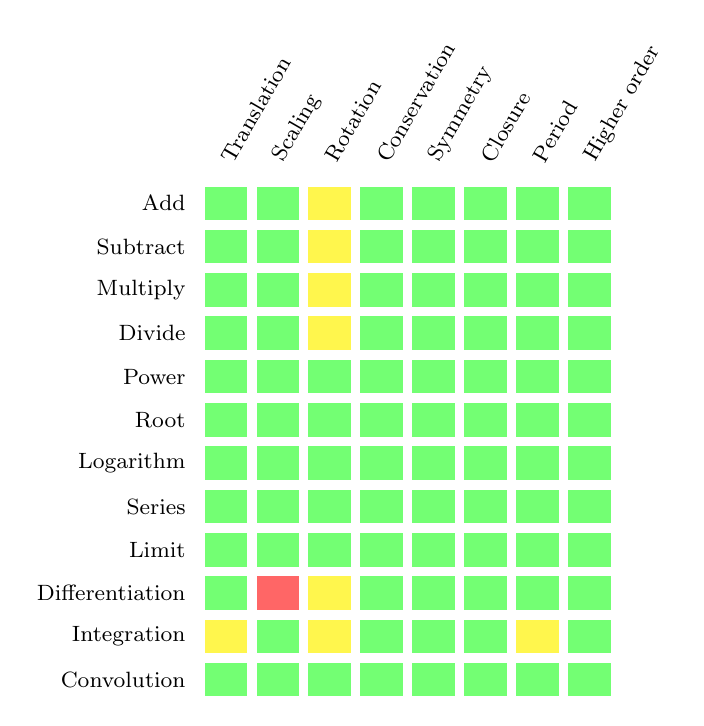
\begin{tikzpicture}[scale=0.55, every node/.style={font=\footnotesize}]
\foreach \r/\vals in {%
  0/{0,0,1,0,0,0,0,0},%
  1/{0,0,1,0,0,0,0,0},%
  2/{0,0,1,0,0,0,0,0},%
  3/{0,0,1,0,0,0,0,0},%
  4/{0,0,0,0,0,0,0,0},%
  5/{0,0,0,0,0,0,0,0},%
  6/{0,0,0,0,0,0,0,0},%
  7/{0,0,0,0,0,0,0,0},%
  8/{0,0,0,0,0,0,0,0},%
  9/{0,2,1,0,0,0,0,0},%
  10/{1,0,1,0,0,0,1,0},%
  11/{0,0,0,0,0,0,0,0}%
} {
  \foreach \val [count=\c from 0] in \vals {
    \ifnum\val=0 \def\col{green!55}\fi
    \ifnum\val=1 \def\col{yellow!70}\fi
    \ifnum\val=2 \def\col{red!60}\fi
    \fill[\col] (\c*1.2, -\r*1.0) rectangle (\c*1.2+1.0, -\r*1.0-0.8);
    \draw[white] (\c*1.2, -\r*1.0) rectangle (\c*1.2+1.0, -\r*1.0-0.8);
  }
}
\node[anchor=east] at (-0.2, -0.4) {Add};
\node[anchor=east] at (-0.2, -1.4) {Subtract};
\node[anchor=east] at (-0.2, -2.4) {Multiply};
\node[anchor=east] at (-0.2, -3.4) {Divide};
\node[anchor=east] at (-0.2, -4.4) {Power};
\node[anchor=east] at (-0.2, -5.4) {Root};
\node[anchor=east] at (-0.2, -6.4) {Logarithm};
\node[anchor=east] at (-0.2, -7.4) {Series};
\node[anchor=east] at (-0.2, -8.4) {Limit};
\node[anchor=east] at (-0.2, -9.4) {Differentiation};
\node[anchor=east] at (-0.2, -10.4) {Integration};
\node[anchor=east] at (-0.2, -11.4) {Convolution};
\foreach \c/\lab in {0/Translation,1/Scaling,2/Rotation,3/Conservation,4/Symmetry,5/Closure,6/Period,7/Higher order} {
  \node[rotate=60, anchor=west] at (\c*1.2+0.4, 0.4) {\lab};
}
\end{tikzpicture}
\caption{Heat map of the transitivity matrix: green indicates complete preservation, yellow indicates preservation under the commensurability or other conditions, and red indicates non-preservation.}
\label{fig:transitivity_matrix_heatmap}
\end{figure}

\begin{remark}[Legend for the transitivity matrix]\label{rem:transitivity_matrix_legend}
\begin{itemize}
    \item $\checkmark$: the property is preserved under the operation.
    \item $\checkmark^*$: the property is preserved under the commensurability condition.
    \item $\checkmark^{**}$: the property is preserved in the sense of modulus (rotation covariance).
    \item $\checkmark^{***}$: the property is preserved under the zero-mean condition ($\int_0^T f = 0$).
    \item $\times$: the property is not preserved (differentiation destroys scaling symmetry).
\end{itemize}
\end{remark}

\begin{theorem}[General pattern of the transitivity matrix]\label{thm:transitivity_pattern}
\begin{enumerate}[label=(\roman*)]
    \item \textbf{Algebraic operations (addition, subtraction, multiplication, division, exponentiation, root extraction, logarithm)}: all properties are preserved. The reason is that pointwise operations commute with the group action.
    \item \textbf{Analytic operations (series, limits)}: all properties are preserved. The reason is that uniform convergence/pointwise convergence guarantees that the group action commutes with the limit.
    \item \textbf{Differentiation}: all are preserved except the scaling property. The reason why differentiation destroys scaling symmetry is that the chain rule introduces an extra scaling factor.
    \item \textbf{Integration}: all are preserved except that the translation/period properties are preserved only conditionally. The reason is that the constant of integration introduces an extra degree of freedom.
    \item \textbf{Convolution}: all are preserved. The reason is that convolution commutes with the group action.
\end{enumerate}
\end{theorem}

\begin{proof}
(i) Representative complete verification (taking multiplication as the example). Let the groups with periodic orbits of $f,g$ be $H_f,H_g$ respectively. For any $h\in H_f\cap H_g$, Lemma \ref{ch8_pointwise_invariance} (taking $\star$ to be multiplication) gives $(fg)(\phi_h(x))=f(\phi_h(x))\,g(\phi_h(x))=f(x)\,g(x)=(fg)(x)$, so $fg$ is invariant under $H_f\cap H_g$ and the property is preserved (Proposition \ref{prop:mult_all}). The objects verified for addition, subtraction, division, exponentiation, root extraction and the logarithm (Proposition \ref{prop:add_all}, \ref{prop:subtraction_all}, \ref{prop:division_all}, \ref{prop:power_all}, \ref{prop:root_all}, \ref{prop:log_all}) are the same---pointwise operations commute with the group action---so they are verified in the same way.

(ii) Verified in the same way: the objects verified are the series and limit operations, and uniform convergence/pointwise convergence guarantees that the group action commutes with $\sum$ and $\lim$ (Proposition \ref{prop:series_all}, \ref{prop:limit_all}).

(iii) The object verified is the differential operator $d/dx$: translation is preserved (Proposition \ref{prop:diff_translation}); scaling is destroyed (Proposition \ref{prop:diff_scaling}, the chain rule introducing the factor $q_0$); rotation is covariant (Proposition \ref{prop:diff_rotation}); the preservation of the remaining properties is verified in the same way from the commutativity of differentiation with the invariance groups.

(iv) The object verified is the integral operator: the translation/period properties are preserved under the zero-mean condition (Proposition \ref{prop:int_translation}), and the scaling/rotation/conservation/symmetry/closure properties are preserved (Proposition \ref{prop:int_all}).

(v) The object verified is convolution: translation is preserved under the commensurability condition (Proposition \ref{prop:conv_translation}) and the remaining seven properties are preserved (Proposition \ref{prop:conv_all}), for the same reason that convolution commutes with the group action.
\end{proof}

\section{\texorpdfstring{The Three Basic Groups and the Corresponding Group Functions}{The Three Basic Groups and the Corresponding Group Functions}}

\subsection{The Translation Group and Translation Functions}

\begin{definition}[Translation group]\label{def:translation_group_basic}
Let $G_{\text{trans}} = \mathbb{R}$ be the additive group. The translation group is the group-representation-theoretic carrier of the translation construction, with infinitesimal generator $\frac{d}{dx}$. Translation invariance implies the conservation of energy (time translation) or of linear momentum (spatial translation).
\end{definition}

\begin{definition}[Translation function]\label{def:translation_function_basic}
If a function $f: \mathbb{R} \to \mathbb{C}$ satisfies $f(x + T_0) = f(x)$, then $f$ is called a \textbf{translation-periodic function} with respect to $\Gamma = T_0\mathbb{Z}$.
\end{definition}

\subsection{The Scaling Group and Scaling Functions}

\begin{definition}[Scaling group]\label{def:scaling_group_basic}
Let $G_{\text{scal}} = \mathbb{R}^+$ be the multiplicative group of positive real numbers. The scaling group is the group-representation-theoretic carrier of the scaling construction, with infinitesimal generator the radial operator $\mathbf{x} \cdot \nabla$.
\end{definition}

\begin{definition}[Scaling function]\label{def:scaling_function_basic}
If a function $f: \mathbb{R}^+ \to \mathbb{C}$ satisfies $f(q_0 x) = f(x)$, then $f$ is called a \textbf{scaling-periodic function} with respect to $\Gamma = \langle q_0 \rangle$. By the logarithmic substitution it is equivalent to a translation function.
\end{definition}

\subsection{The Rotation Group and Rotation Functions}

\begin{definition}[Rotation group]\label{def:rotation_group_basic}
Let $G_{\text{rot}} = U(1)$ be the one-dimensional unitary group. The rotation group is one of the group-representation-theoretic carriers of inner automorphisms.
\end{definition}

\begin{definition}[Rotation function]\label{def:rotation_function_basic}
If a function $f: \mathbb{C} \to \mathbb{C}$ satisfies $f(e^{i\theta_0} z) = f(z)$, then $f$ is called a \textbf{rotation-periodic function} with respect to $\Gamma = \langle e^{i\theta_0} \rangle$.
\end{definition}

\subsection{The Unified Duality of the Three Groups}

\begin{theorem}[Unified duality theorem for the three groups]\label{thm:three_groups_duality}
The three basic groups stand in the following correspondence under Pontryagin duality:
\begin{center}
\begin{tabular}{>{\centering\arraybackslash}p{2.2cm}>{\centering\arraybackslash}p{2.2cm}>{\centering\arraybackslash}p{2.5cm}>{\centering\arraybackslash}p{2.5cm}>{\centering\arraybackslash}p{3cm}}
\toprule
Group type & Group $G$ & Period subgroup & Quotient space & Pontryagin dual \\
\midrule
Translation group & $\mathbb{R}$ & $T_0\mathbb{Z}$ & $\mathbb{R}/T_0\mathbb{Z} \cong S^1$ & $\widehat{S^1} \cong \mathbb{Z}$ \\
Scaling group & $\mathbb{R}^+ \cong \mathbb{R}$ & $\langle q_0 \rangle$ & $\mathbb{R}^+/\langle q_0 \rangle \cong S^1$ & $\widehat{S^1} \cong \mathbb{Z}$ \\
Rotation group & $U(1) \cong S^1$ & $\langle e^{i\theta_0} \rangle$ & $U(1)/C_n \cong U(1)$ & $\widehat{U(1)} \cong \mathbb{Z}$ \\
\bottomrule
\end{tabular}
\end{center}
\end{theorem}

\begin{proof}
Verify row by row. Translation row: the mapping $\chi(x)=e^{2\pi i x/T_0}$ is a surjective homomorphism $\mathbb{R}\to S^1$ whose kernel is exactly $T_0\mathbb{Z}$, hence $\mathbb{R}/T_0\mathbb{Z}\cong S^1$; the family of characters of $S^1$, $\{\chi_n:e^{i\theta}\mapsto e^{in\theta}\mid n\in\mathbb{Z}\}$, gives $\widehat{S^1}\cong\mathbb{Z}$. Scaling row: the logarithm mapping $x\mapsto\ln x$ is an isomorphism $\mathbb{R}^+\cong\mathbb{R}$ and maps $\langle q_0\rangle$ to $(\ln q_0)\mathbb{Z}$, hence is isomorphic to the translation row, with quotient $\cong S^1$ and dual $\cong\mathbb{Z}$. Rotation row: $U(1)\cong S^1$; when $\theta_0/(2\pi)=p/q$, $\langle e^{i\theta_0}\rangle\cong C_q$, and the kernel of the mapping $z\mapsto z^q$ is the group of $q$-th roots of unity $C_q$, hence $U(1)/C_q\cong U(1)$; the characters $\chi_n(z)=z^n$ give $\widehat{U(1)}\cong\mathbb{Z}$. The duals in all three rows are $\cong\mathbb{Z}$, so the table holds.
\end{proof}

\begin{figure}[htbp]
\centering
\begin{tikzpicture}[>=Stealth, thick, node distance=2.0cm, scale=0.95, every node/.style={transform shape}]

\node[draw, rounded corners, fill=blue!8, align=center, minimum width=2.4cm, minimum height=0.9cm] (trans) {translation group\\$\mathbb{R}$};
\node[draw, rounded corners, fill=green!8, align=center, minimum width=2.4cm, minimum height=0.9cm, below=of trans] (scal) {scaling group\\$\mathbb{R}^+\cong\mathbb{R}$};
\node[draw, rounded corners, fill=orange!8, align=center, minimum width=2.4cm, minimum height=0.9cm, below=of scal] (rot) {rotation group\\$U(1)\cong S^1$};

\node[draw, rounded corners, fill=purple!8, align=center, minimum width=2.6cm, minimum height=0.9cm] (dual) at (6, -2) {dual group\\$\widehat{G}\cong\mathbb{Z}$};

\draw[->] (trans.east) -- (dual.north west) node[midway, above, sloped, font=\footnotesize] {logarithm mapping};
\draw[->] (scal.east) -- (dual.west) node[pos=0.5, above, font=\footnotesize, xshift=-0.3cm, yshift=0.3cm] {Fourier duality};
\draw[->] (rot.east) -- (dual.south west) node[midway, below, sloped, font=\footnotesize] {character $z\mapsto z^n$};

\end{tikzpicture}
\caption{Pontryagin duality relations of the three basic groups: the translation group, the scaling group and the rotation group are unified as $\mathbb{Z}$ under duality, constituting three representations of a unified algebraic structure}
\label{fig:three_groups_duality}
\end{figure}

\begin{corollary}[The three functions, groups, fixed points and conservation laws]\label{cor:three_functions_trinity}
\begin{center}
\begin{tabular}{>{\centering\arraybackslash}p{2.2cm}>{\centering\arraybackslash}p{2cm}>{\centering\arraybackslash}p{1.8cm}>{\centering\arraybackslash}p{2.2cm}>{\centering\arraybackslash}p{2.2cm}}
\toprule
Function type & Group & Fixed element & Formally corresponding conservation law & Formally corresponding flux \\
\midrule
Translation function & $\mathbb{R}$ & $0$ & Energy/linear momentum & Time flux \\
Scaling function & $\mathbb{R}^+$ & $1$ & Scale charge & Observation flux \\
Rotation function & $U(1)$ & $i$ & Angular momentum & Spatial flux \\
\bottomrule
\end{tabular}
\end{center}
The two columns `formally corresponding conservation law' and `formally corresponding flux' in the table give a conceptual comparison between objects of group representation theory and physical concepts.
\end{corollary}

\begin{proof}
By Definition \ref{def:translation_function_basic}, \ref{def:scaling_function_basic} and \ref{def:rotation_function_basic}, the translation function, the scaling function and the rotation function have $\mathbb{R}$, $\mathbb{R}^+$ and $U(1)$ respectively as their acting groups, with period subgroups $T_0\mathbb{Z}$, $\langle q_0\rangle$ and $\langle e^{i\theta_0}\rangle$ in that order. The fixed elements are the reference points of the three cases $0$, $1$ and $i$ respectively. The correspondence between conservation laws and fluxes is as in Proposition \ref{prop:translation_operator}, \ref{prop:scaling_operator} and \ref{prop:rotation_operator}. The quotient spaces and Pontryagin duality are given by Theorem \ref{thm:three_groups_duality}.
\end{proof}

\section{\texorpdfstring{A unified perspective on group functions and periodic mathematics}{A unified perspective on group functions and periodic mathematics}}

\begin{remark}[The place of group functions in periodic mathematics]\label{rem:group_function_hub}
This chapter obtains a unified formulation, at the level of group representation theory, of the core concepts of periodic mathematics:
\begin{enumerate}[label=(\roman*)]
    \item \textbf{The automorphism tower}: the automorphism tower realises `the higher-order relation of a relation is again a group'.
    \item \textbf{The three constructions on a group}: translation, inner automorphism, outer automorphism.
    \item \textbf{The eight pairs of concepts}: precise definitions of the translation/scaling/rotation/conservation/symmetry/closure/period/higher-order functions and groups.
    \item \textbf{The joint phase-space criterion}: the unification of the group representation theory criterion + the phase-space criterion + the conservation criterion.
    \item \textbf{The transitivity matrix}: a complete transitivity analysis of the eight properties under the twelve operations.
    \item \textbf{Group functions---regular representation and characters}: the representation decomposition of $L^2(G)$.
\end{enumerate}
\end{remark}

\begin{figure}[htbp]
    \centering
    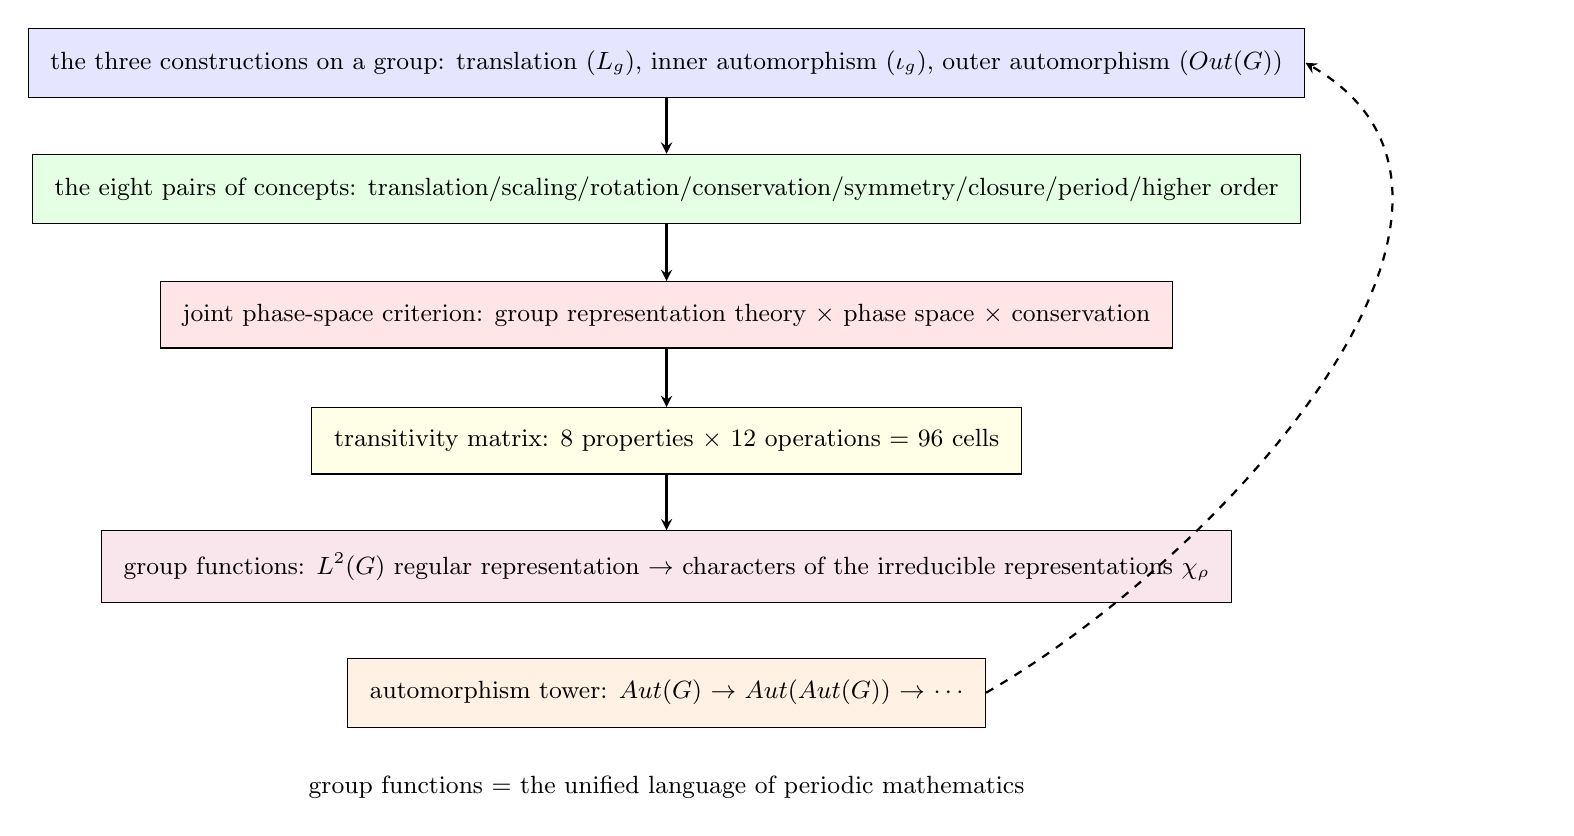
\begin{tikzpicture}[scale=1.0,>=stealth,
        box/.style={draw,rectangle,minimum width=8cm,inner sep=8pt,font=\small}]
        \node[box,fill=blue!10] (ops) at (0,0) {the three constructions on a group: translation ($L_g$), inner automorphism ($\iota_g$), outer automorphism ($\operatorname{Out}(G)$)};
        \node[box,fill=green!10] (conc) at (0,-1.6) {the eight pairs of concepts: translation/scaling/rotation/conservation/symmetry/closure/period/higher order};
        \node[box,fill=red!10] (phase) at (0,-3.2) {joint phase-space criterion: group representation theory $\times$ phase space $\times$ conservation};
        \node[box,fill=yellow!10] (matrix) at (0,-4.8) {transitivity matrix: 8 properties $\times$ 12 operations $=$ 96 cells};
        \node[box,fill=purple!10] (func) at (0,-6.4) {group functions: $L^2(G)$ regular representation $\to$ characters of the irreducible representations $\chi_\rho$};
        \node[box,fill=orange!10] (higher) at (0,-8.0) {automorphism tower: $\operatorname{Aut}(G)$ $\to$ $\operatorname{Aut}(\operatorname{Aut}(G))$ $\to$ $\cdots$};
        
        \draw[->,thick] (ops) -- (conc);
        \draw[->,thick] (conc) -- (phase);
        \draw[->,thick] (phase) -- (matrix);
        \draw[->,thick] (matrix) -- (func);
        \draw[->,thick,dashed] (higher.east) to[out=30,in=330] (ops.east);
        
        \node[font=\small] at (0,-9.2) {group functions = the unified language of periodic mathematics};
    \end{tikzpicture}
    \caption{The complete system of groups and group functions.}
    \label{fig:group_function_hierarchy}
\end{figure}

\section*{Seven-theme comparison table for this chapter}

\begin{center}
\renewcommand{\arraystretch}{1.3}
\begin{tabular}{>{\centering\arraybackslash}p{2.2cm}>{\centering\arraybackslash}p{10.5cm}}
\toprule
Theme & Corresponding content in this chapter \\
\midrule
Translation & The translation construction on a group (Definition \ref{def:group_translation_operation}) and its basic properties (Proposition \ref{prop:translation_operator}); the translation group/translation function pair of concepts \\
Scaling & The outer automorphism on a group (Definition \ref{def:group_scaling_operation}) and its basic properties (Proposition \ref{prop:scaling_operator}); the scaling group/scaling function pair of concepts \\
Rotation & The inner automorphism on a group (Definition \ref{def:group_rotation_operation}) and its basic properties (Proposition \ref{prop:rotation_operator}); the rotation group/rotation function pair of concepts \\
Conservation & The group--fixed element--conservation law comparison of the three constructions (Remark \ref{cor:three_functions_trinity}); the conservation group/conservation function pair of concepts \\
Symmetry & Translational symmetry and automorphism symmetry (Definition \ref{def:group_translation_symmetry}, \ref{def:group_automorphism_symmetry}), the automorphism tower (Definition \ref{def:automorphism_tower}), and the symmetry group/symmetry function pair of concepts \\
Closure & The closure of finite orbits in the orbit-stabiliser theorem (Theorem \ref{thm:orbit_stabilizer}); the closure group/closure function pair of concepts; the joint phase-space and group-theoretic criterion for the periodicity of a function (Theorem \ref{thm:phase_group_joint_criterion}) \\
Period & The group period (Definition \ref{def:group_strict_period}) and its basic properties (Proposition \ref{prop:group_period_properties}); the group with periodic orbits/periodic function pair of concepts; the transitivity matrix (Table \ref{tab:transitivity_matrix}) and its general pattern (Theorem \ref{thm:transitivity_pattern}) \\
\bottomrule
\end{tabular}
\end{center}

\section*{Exercises}

\begin{enumerate}[leftmargin=3em, label=\textbf{Exercise \arabic*}]
    \item By Definition \ref{def:group_translation_operation}, verify the three basic properties of left and right translation:
    \begin{enumerate}[label=(\roman*)]
        \item $L_g\circ L_h=L_{gh}$, and $\{L_g\}\cong G$ (the left regular action);
        \item $R_g\circ R_h=R_{hg}$, and $\{R_g\}\cong G^{\text{op}}$;
        \item $L_g\circ R_h=R_h\circ L_g$.
    \end{enumerate}
    Also explain why, when $G$ is non-commutative, the left translation group and the right translation group are in general different as subgroups of $G$.

    \item Prove the four properties of the translation construction in Proposition \ref{prop:translation_operator}:
    fixed elements, infinitesimal generators, invariance of the Haar measure and directional structure.
    Taking $G=\mathbb{Z}$, $G=\mathbb{R}$ and $G=GL(n,\mathbb{R})$ as examples respectively,
    verify the concrete forms of left and right translation.

    \item Prove the four properties of inner automorphisms in Proposition \ref{prop:rotation_operator}:
    the fixed elements are the centre $Z(G)$, the infinitesimal generator is the adjoint representation, the conserved quantity is a class function, and adjoint orbits.
    Verify that $\iota_g$ is an automorphism and that the kernel of the mapping $g\mapsto\iota_g$ is $Z(G)$,
    and explain why all inner automorphisms are the identity mapping when $G=U(1)$.

    \item Verify the three examples of inner automorphisms in Example \ref{ex:rotation_operation_examples}:
    \begin{enumerate}[label=(\roman*)]
        \item the similarity transformation $\iota_A(X)=AXA^{-1}$ in $GL(n,\mathbb{R})$;
        \item the conjugation of a rotation in $SO(3)$ into a rotation about a new axis;
        \item the degeneration of inner automorphisms to the identity in $U(1)$.
    \end{enumerate}
    Taking $A=\operatorname{diag}(2,1)$ and the permutation matrix $P$,
    compute $PAP^{-1}$ and verify that the eigenvalues are invariant under conjugation.

    \item Prove the four properties of outer automorphisms in Proposition \ref{prop:scaling_operator},
    and verify Example \ref{ex:scaling_operation_examples}:
    \begin{enumerate}[label=(\roman*)]
        \item $\operatorname{Aut}(\mathbb{Z})\cong C_2=\{\operatorname{id},-\operatorname{id}\}$;
        \item $\operatorname{Aut}(C_n)\cong(\mathbb{Z}/n\mathbb{Z})^\times$, of order $\varphi(n)$;
        \item $\operatorname{Aut}(\mathbb{R}^+)\cong\mathbb{R}^\times$, with automorphisms $x\mapsto x^\lambda$.
    \end{enumerate}
    Compute the order and the generators of $\operatorname{Aut}(C_5)$ when $n=5$.

    \item Prove Theorem \ref{thm:three_operations_unity}:
    the three standard constructions on a group form the following structure in the automorphism group $\operatorname{Aut}(G)$:
    translation is realised by the left regular action, the inner automorphism group is $\operatorname{Inn}(G)\cong G/Z(G)$,
    and the outer automorphism group is $\operatorname{Out}(G)=\operatorname{Aut}(G)/\operatorname{Inn}(G)$.
    Write down the exact sequence
    \[
    1\to Z(G)\to G\xrightarrow{\phi}\operatorname{Aut}(G)
    \xrightarrow{\pi}\operatorname{Out}(G)\to 1,
    \]
    and verify its exactness term by term.

    \item Prove Lemma \ref{ch8_centreless_embedding}:
    let $G$ be a finite group with $Z(G)=\{e\}$; then
    \begin{enumerate}[label=(\roman*)]
        \item $G\cong\operatorname{Inn}(G)\subseteq\operatorname{Aut}(G)$, and therefore $|G|\le|\operatorname{Aut}(G)|$;
        \item if $|\operatorname{Aut}(G)|=|G|$, then $\operatorname{Aut}(G)=\operatorname{Inn}(G)\cong G$;
        \item $Z(\operatorname{Aut}(G))=\{e\}$, that is, triviality of the centre is preserved level by level.
    \end{enumerate}

    \item Verify the automorphism tower heights of the typical groups in Proposition \ref{prop:tower_heights}:
    \begin{enumerate}[label=(\roman*)]
        \item $C_2\to\{e\}$, height $1$;
        \item $C_3\to C_2\to\{e\}$, height $2$;
        \item $C_5\to C_4\to C_2\to\{e\}$, height $3$;
        \item $S_3\to S_3$, height $0$.
    \end{enumerate}
    Compute the automorphism group of each level, and explain why the outer automorphism group of $S_3$ is the trivial group.

    \item Prove Theorem \ref{thm:orbit_stabilizer} (the orbit-stabiliser theorem):
    if a finite group $G$ acts on a finite set $X$, then for any $x\in X$,
    \[
    |G\cdot x|=\frac{|G|}{|G_x|}.
    \]
    Complete the proof by constructing a bijection $G/G_x\to G\cdot x$,
    and explain how this theorem characterises the closure of finite orbits.

    \item Prove Proposition \ref{prop:translation_automorphism_compatibility}:
    if $\varphi\in\operatorname{Aut}(G)$ and $g\in G$, then
    \[
    \varphi\circ L_g\circ\varphi^{-1}=L_{\varphi(g)}.
    \]
    Also explain why outer automorphisms do not preserve the conjugacy-class structure whereas inner automorphisms do.

    \item Starting from Definition \ref{def:translation_function_gf} through to Definition \ref{def:higher_group_gf},
    write out the definitions of the eight pairs of concepts, and verify Proposition \ref{prop:invariance_subgroup_structure}:
    \begin{enumerate}[label=(\roman*)]
        \item $\operatorname{Group}_{\mathrm{period}}(f)=\operatorname{Symmetry}(f)$;
        \item $\operatorname{Symmetry}(f)\subseteq\operatorname{Group}_{\mathrm{conservation}}(f,Q)$;
        \item the translation group, the scaling group and the rotation group are all contained in $\operatorname{Symmetry}(f)$;
        \item the higher-order group and the higher-order functions are related level by level through the automorphism tower.
    \end{enumerate}

    \item Prove Theorem \ref{thm:phase_group_joint_criterion}:
    let $f$ be a smooth function and let $G$ act on its domain; then $f$ is a periodic function with respect to $g\in G$ if and only if the phase-space trajectory satisfies $\Gamma_f(\phi_g(x))=\Gamma_f(x)$.
    Prove the two directions separately, and explain why (i) $g\in\operatorname{Group}_{\mathrm{period}}(f)$ and (iii) `there exists a conserved quantity $Q$ such that $Q(f(x))$ is constant along $\Gamma_f$' are not conditions independent of, and on a par with, (ii)---show how (ii) implies (i) and (iii), and why (iii) cannot imply (ii).

    \item Prove the three basic properties of group periodicity in Proposition \ref{prop:group_period_properties}:
    \begin{enumerate}[label=(\roman*)]
        \item period closure: $\gamma_1,\gamma_2\in\Gamma\Rightarrow\gamma_1\gamma_2\in\Gamma$;
        \item the $L^2$ integrability condition: if $f\neq0$ and $f\in L^2(G)$, then $\Gamma$ is a finite subgroup;
        \item determination by the fundamental domain: the values of $f$ on a fundamental domain completely determine $f$.
    \end{enumerate}

    \item Prove Proposition \ref{prop:regular_unitary}:
    the left regular representation and the right regular representation on a locally compact group $G$ are both unitary representations on $L^2(G)$.
    Complete the proof using respectively the left invariance and the right invariance of the left Haar measure.

    \item Prove Theorem \ref{thm:class_function_expansion} (the class-function version of the Peter--Weyl theorem):
    let $G$ be a compact group; then the characters $\{\chi_\rho\}$ of the irreducible unitary representations form
    a complete orthogonal basis of $L^2(G)_{\text{class}}$.
    Write out the proof of the Schur orthogonality relations, and explain how an arbitrary class function is expanded as a series of characters.

    \item Prove Proposition \ref{prop:convolution_orbit}:
    let $G$ be a compact group and $K$ a class function; then the convolution operator $C_K f=K*f$ is diagonalised under the orbit decomposition:
    \[
    (C_K f)_\rho=\frac{\hat{K}(\rho)}{\dim\rho}f_\rho,
    \quad
    \hat{K}(\rho)=\langle K,\chi_\rho\rangle.
    \]
    Complete the proof using the Schur orthogonality relations.

    \item Prove Theorem \ref{thm:automorphic_quotient}:
    automorphic functions are equivalent to sections of the quotient space $\Gamma\backslash(G\times V)$.
    Write out the constructions in the two directions, `from automorphic functions to sections' and `from sections to automorphic functions',
    and verify that the two are mutually inverse.

    \item Prove Lemma \ref{ch8_pointwise_invariance}:
    let $f,g$ be functions invariant under the subgroups $H_f,H_g$ respectively
    and let $\star$ be a pointwise binary operation; then
    \begin{enumerate}[label=(\roman*)]
        \item $f\star g$ is invariant under $H_f\cap H_g$;
        \item for any pointwise unary operation $\triangle$, $\triangle f$ is invariant under $H_f$.
    \end{enumerate}
    Explain why this lemma is the unified basis of proof for the algebraic-operation cells of the transitivity matrix.

    \item Verify Proposition \ref{prop:add_translation} and Proposition \ref{ch8_add_scaling}:
    \begin{enumerate}[label=(\roman*)]
        \item if the translation groups of $f,g$ are $T_f\mathbb{Z}$ and $T_g\mathbb{Z}$ respectively,
              then $f+g$ has period $\operatorname{lcm}(T_f,T_g)$ whenever $T_f/T_g\in\mathbb{Q}$;
        \item if the scaling groups of $f,g$ are $\langle q_f\rangle$ and $\langle q_g\rangle$ respectively,
              then $f\pm g$ and $fg$ are still scaling functions whenever $\ln q_f/\ln q_g\in\mathbb{Q}$.
    \end{enumerate}
    Explain why the commensurability condition is a necessary condition for the preservation of periodic structure.

    \item Prove Proposition \ref{prop:diff_scaling} and Proposition \ref{prop:diff_rotation}:
    \begin{enumerate}[label=(\roman*)]
        \item differentiation destroys scaling symmetry: if $f(q_0x)=f(x)$, then
              $f'(q_0x)=f'(x)/q_0\neq f'(x)$;
        \item the rotation property is preserved covariantly under differentiation: if $f(e^{i\theta}z)=f(z)$, then
              $f'(e^{i\theta}z)=e^{-i\theta}f'(z)$, and $|f'|$ is a rotation function.
    \end{enumerate}
    Explain why the extra scaling factor introduced by the chain rule is the fundamental reason why differentiation destroys scaling symmetry.

    \item Prove Proposition \ref{prop:int_translation}:
    let $f$ be a continuous translation function and $F(x)=\int_0^x f(t)\,dt$;
    then $F$ is a translation function if and only if $\int_0^Tf(t)\,dt=0$.
    Write out the proof, and explain why the extra degree of freedom introduced by the constant of integration causes the translation property to be preserved only conditionally.

    \item Prove Theorem \ref{thm:transitivity_pattern}:
    the general pattern of the transitivity matrix:
    \begin{enumerate}[label=(\roman*)]
        \item algebraic operations (addition, subtraction, multiplication, division, exponentiation, root extraction, logarithm): all properties are preserved;
        \item analytic operations (series, limits): all properties are preserved;
        \item differentiation: all are preserved except the scaling property;
        \item integration: all are preserved except that the translation/period properties are preserved only conditionally;
        \item convolution: all are preserved.
    \end{enumerate}
    Point out separately the reason why each class of operations preserves or fails to preserve the properties.

    \item Prove Theorem \ref{thm:three_groups_duality}:
    the three basic groups stand in correspondence under Pontryagin duality:
    \begin{enumerate}[label=(\roman*)]
        \item $\mathbb{R}/T_0\mathbb{Z}\cong S^1$, $\widehat{S^1}\cong\mathbb{Z}$;
        \item $\mathbb{R}^+/\langle q_0\rangle\cong S^1$, with dual isomorphic to $\mathbb{Z}$;
        \item $U(1)/C_n\cong U(1)$, $\widehat{U(1)}\cong\mathbb{Z}$.
    \end{enumerate}
    Verify the quotient-space structure and the dual-group structure of the three rows separately.

    \item Synthesis: combining the three standard constructions on a group (Definition \ref{def:group_translation_operation},
    \ref{def:group_rotation_operation}, \ref{def:group_scaling_operation}),
    the eight pairs of concepts (\S\ref{sec:group_function_basic}),
    the joint phase-space criterion framework (Theorem \ref{thm:phase_group_joint_criterion})
    and the transitivity matrix (Table \ref{tab:transitivity_matrix}),
    explain how groups and group functions provide a unified algebraic language for periodic mathematics.
    Point out separately:
    \begin{enumerate}[label=(\roman*)]
        \item how the three standard constructions correspond to translation, scaling and rotation respectively;
        \item how the eight pairs of concepts characterise the hierarchy of periodic structure;
        \item how the transitivity matrix summarises the preservation pattern of the eight properties under the twelve operations;
        \item how the automorphism tower realises `the higher-order relation of a relation is again a group'.
    \end{enumerate}
\end{enumerate}
